\chapter{Diseño Conceptual (PIM)}

\section{El Modelo Independiente de Plataforma}

El Diseño Conceptual representa la fase de traducción y especialización técnica dentro del flujo \textit{MDAA}. En esta etapa, el usuario elabora el \textit{PIM} (\textit{Platform Independent Model}), donde los requerimientos puramente musicales del \textit{CIM} se enriquecen con conceptos computacionales y arquitectónicos, aunque manteniéndose independientes de la tecnología final de despliegue.

\begin{figure}[!ht]
    \centering
    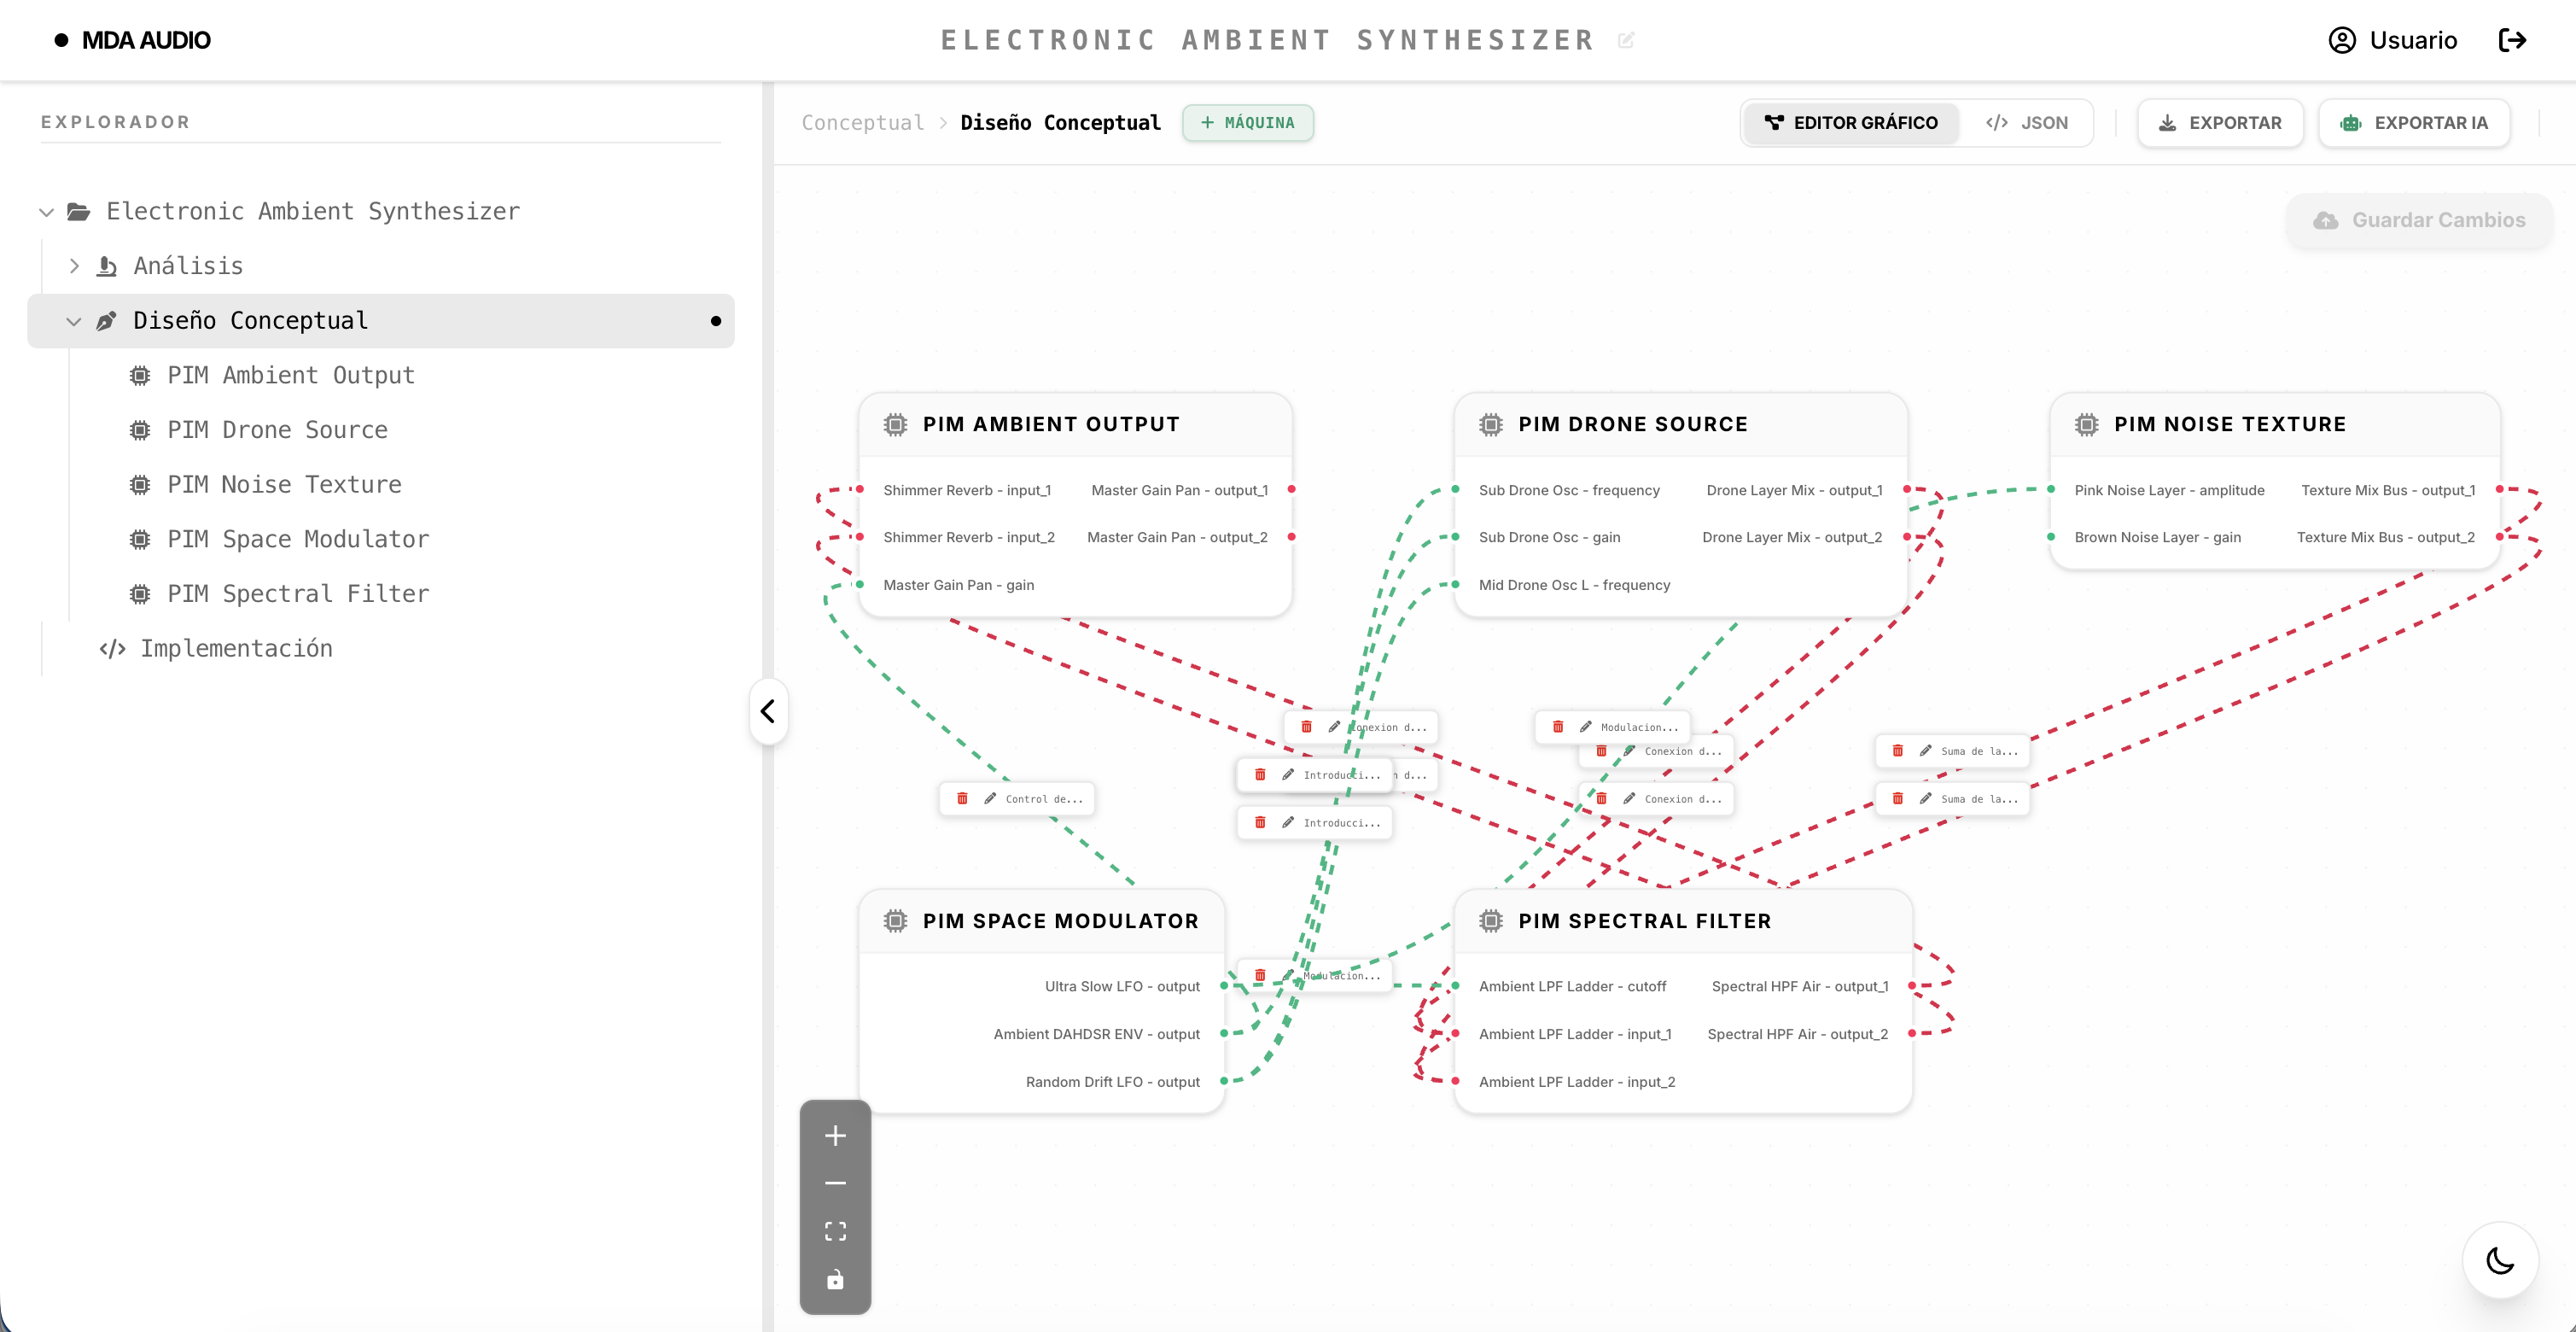
\includegraphics[width=\textwidth]{imagenes/06_diseno/01_pantallaDisenoConceptual.png}
    \caption{Vista general del entorno de Diseño Conceptual.}
\end{figure}

Al navegar a la sección de Diseño Conceptual, la aplicación presenta herramientas destinadas a vincular y mapear las construcciones teóricas hacia estructuras de diseño de software (ej. componentes, bloques de procesamiento de audio).

\begin{figure}[!ht]
    \centering
    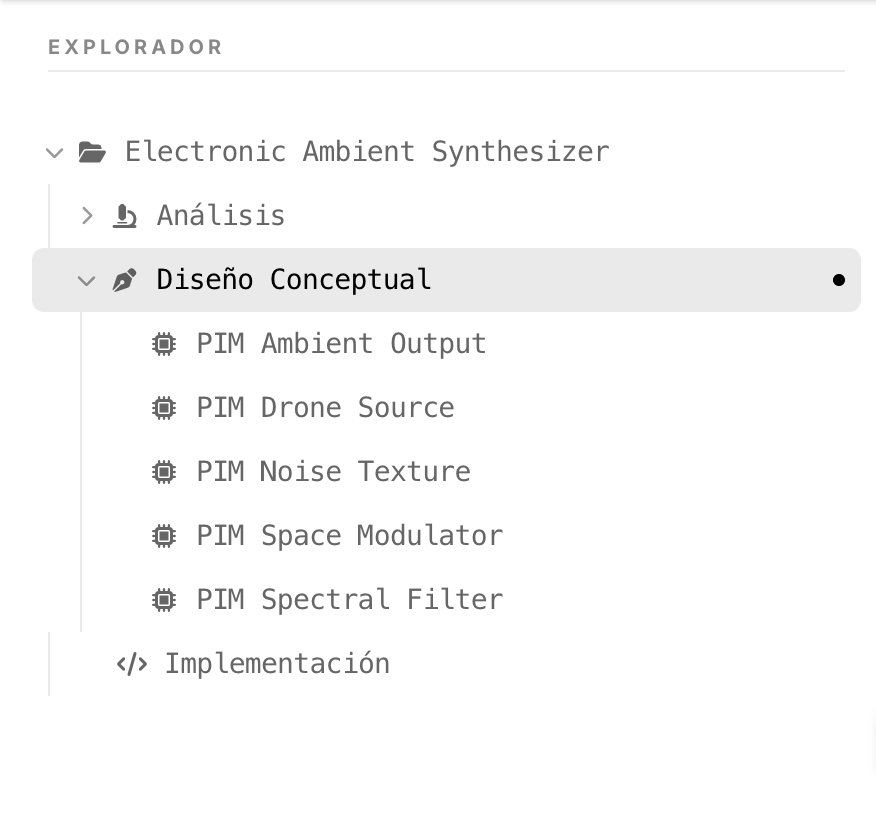
\includegraphics[width=0.4\textwidth]{imagenes/06_diseno/02_exploradorDisenoConceptual.png}
    \caption{Detalle de la rama de Diseño Conceptual en el explorador.}
\end{figure}

De modo paralelo al \textit{CIM}, el árbol del \textit{PIM} organiza las máquinas de diseño y las relaciones globales que definen el ecosistema orquestal desde una perspectiva de arquitectura de software.

\subsection{Creación y Gestión de Máquinas PIM}

\begin{figure}[!ht]
    \centering
    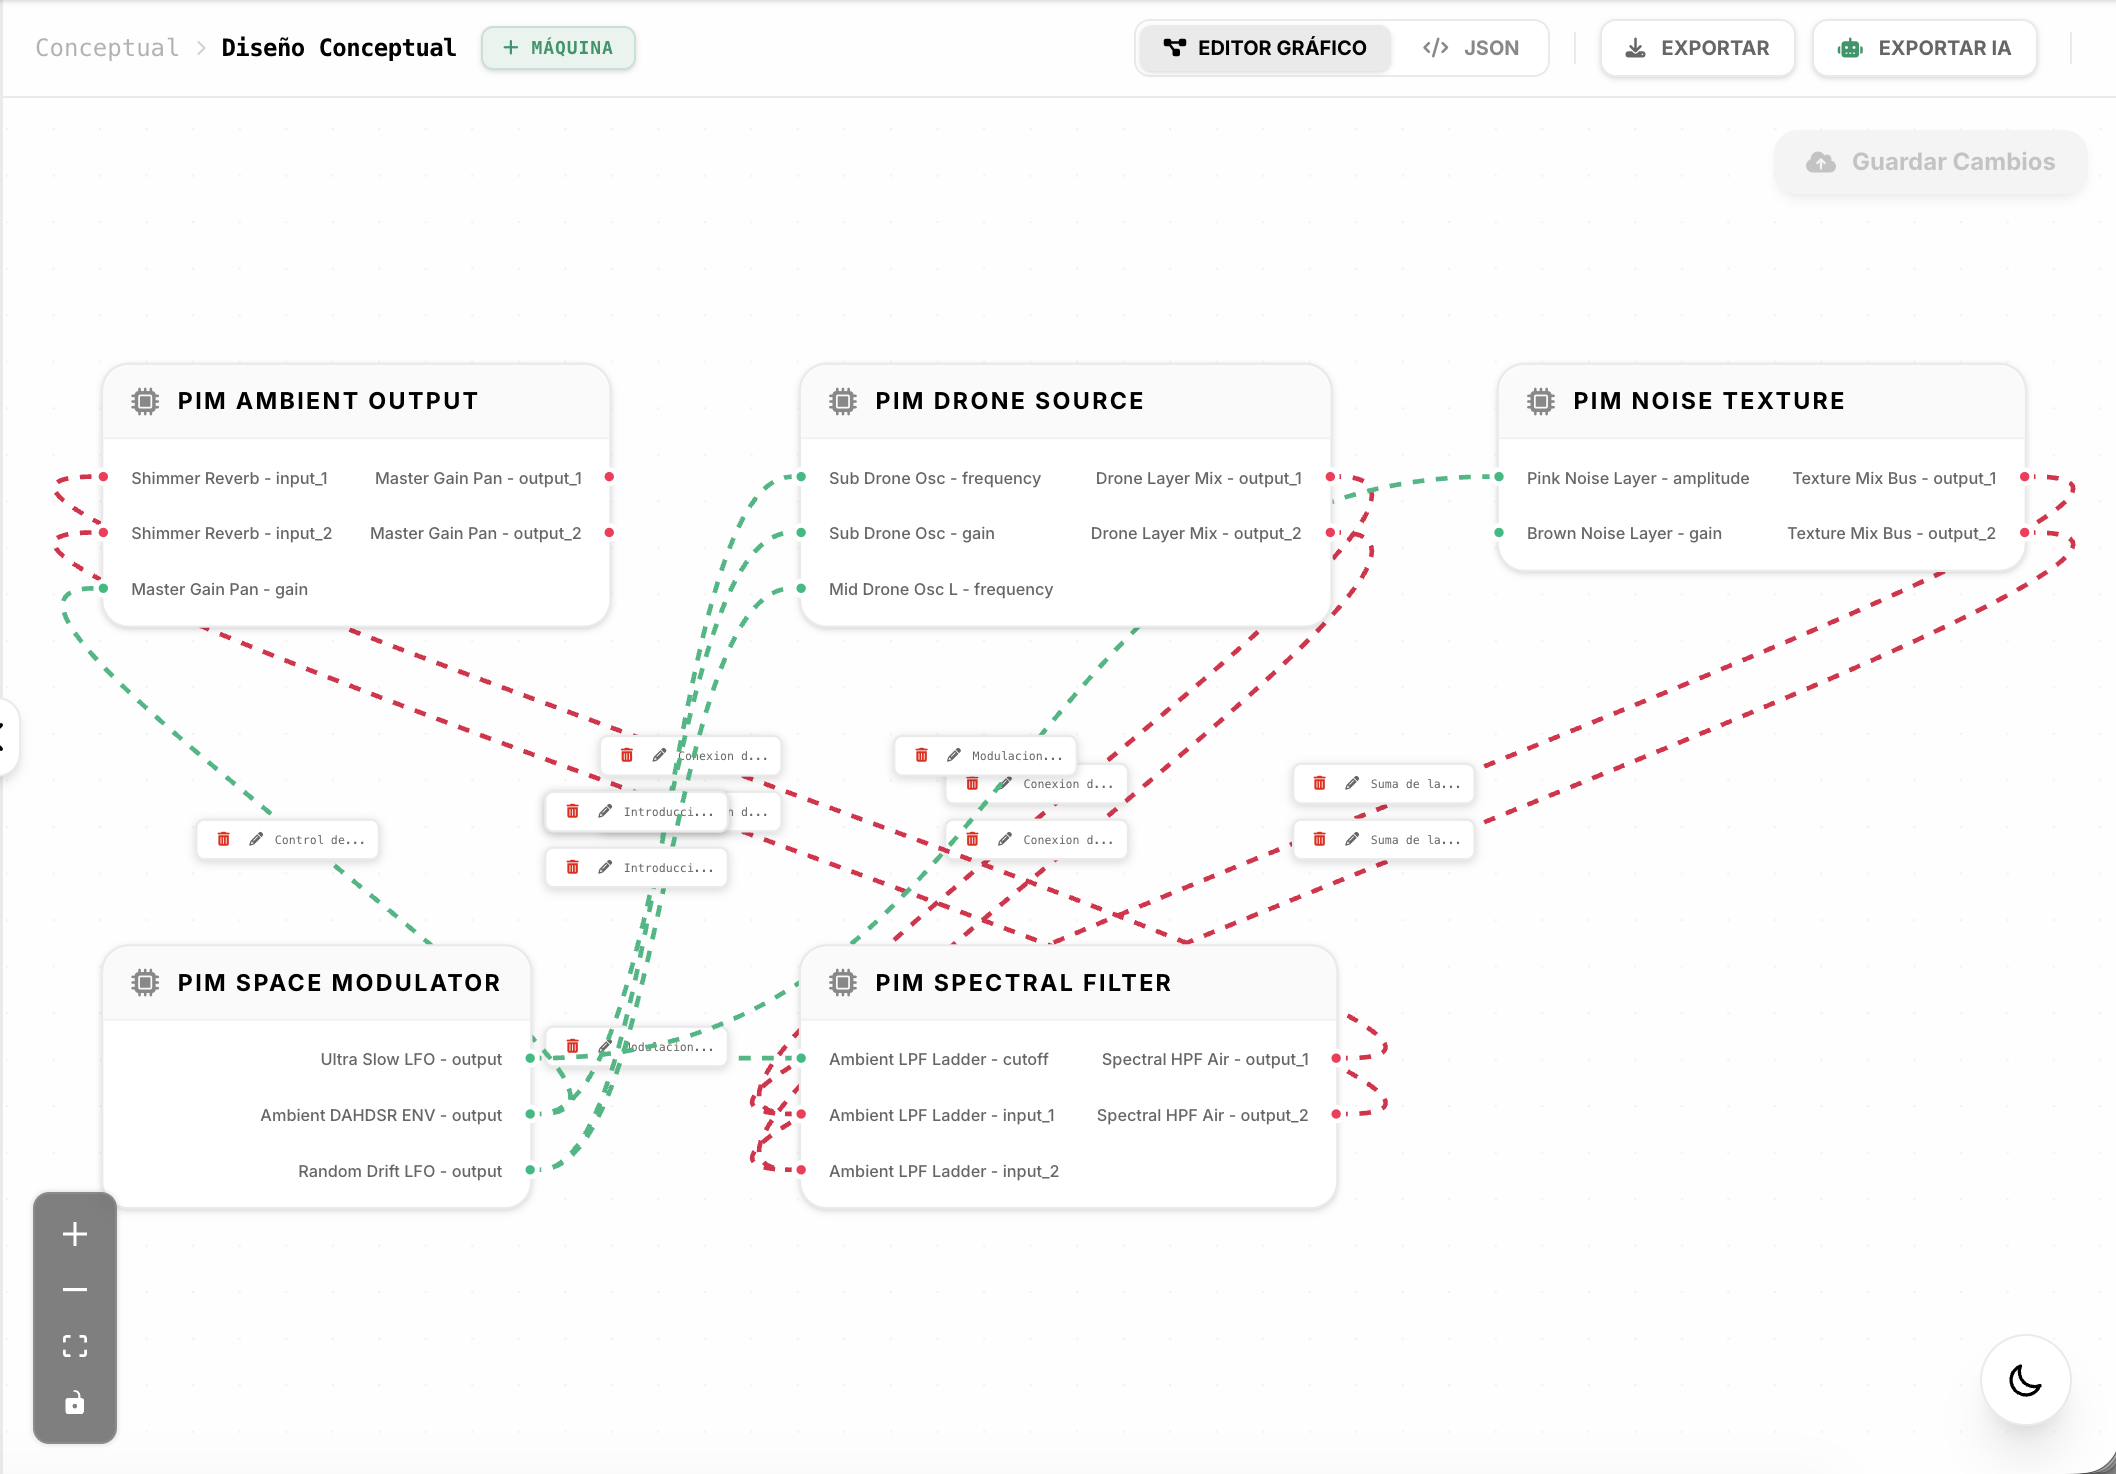
\includegraphics[width=\textwidth]{imagenes/06_diseno/03_visorEditorRelacionesPIM.png}
    \caption{Editor principal de relaciones en el nivel de Diseño Conceptual.}
\end{figure}

\begin{figure}[!ht]
    \centering
    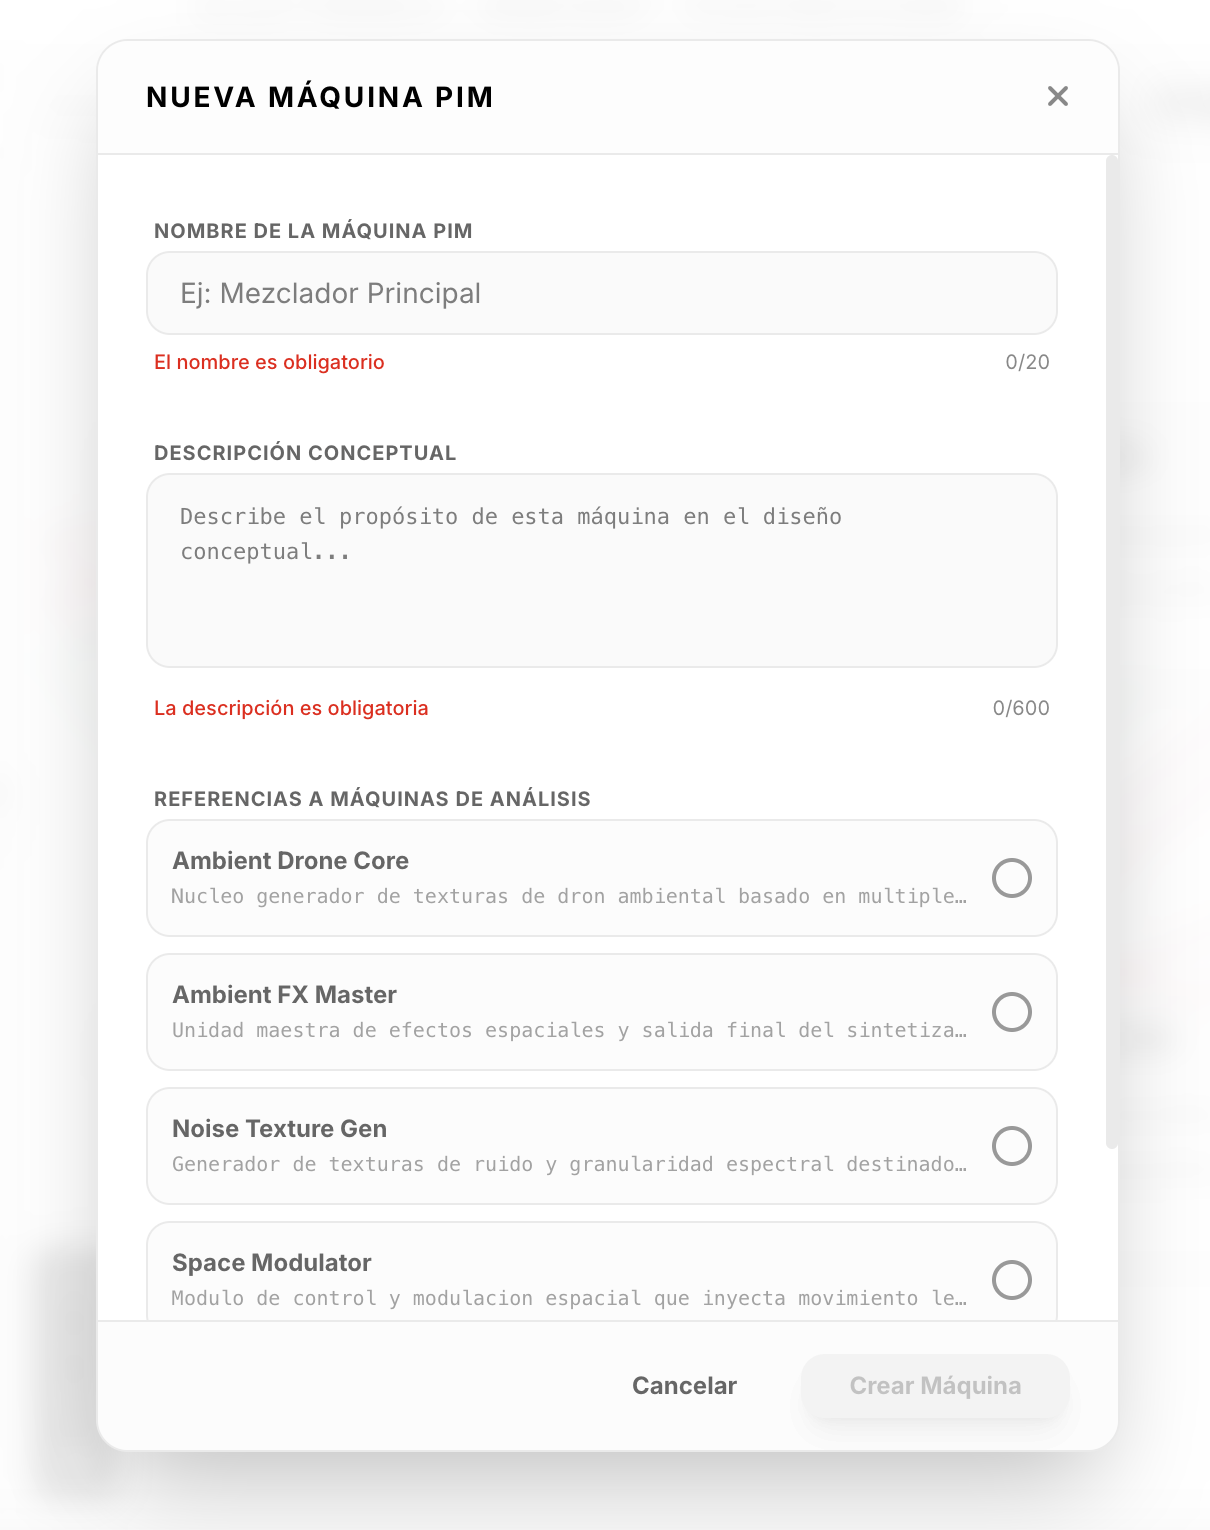
\includegraphics[width=0.6\textwidth]{imagenes/06_diseno/04_formularioCrearNuevaMaquinaPim.png}
    \caption{Formulario de instanciación de una nueva máquina PIM.}
\end{figure}

Desde el editor de relaciones del nivel \textit{PIM}, es posible crear nuevas máquinas de diseño. Crucialmente, estas máquinas \textit{PIM} a menudo referencian y especializan a las máquinas \textit{CIM} subyacentes, estableciendo el puente entre análisis y diseño definido por el lenguaje \textit{DSL}.

\section{Edición de Relaciones PIM}

La interactividad y la edición avanzada son pilares fundamentales para establecer la red de diseño computacional.

\subsection{Visor Gráfico y Edición Topológica}

\begin{figure}[!ht]
    \centering
    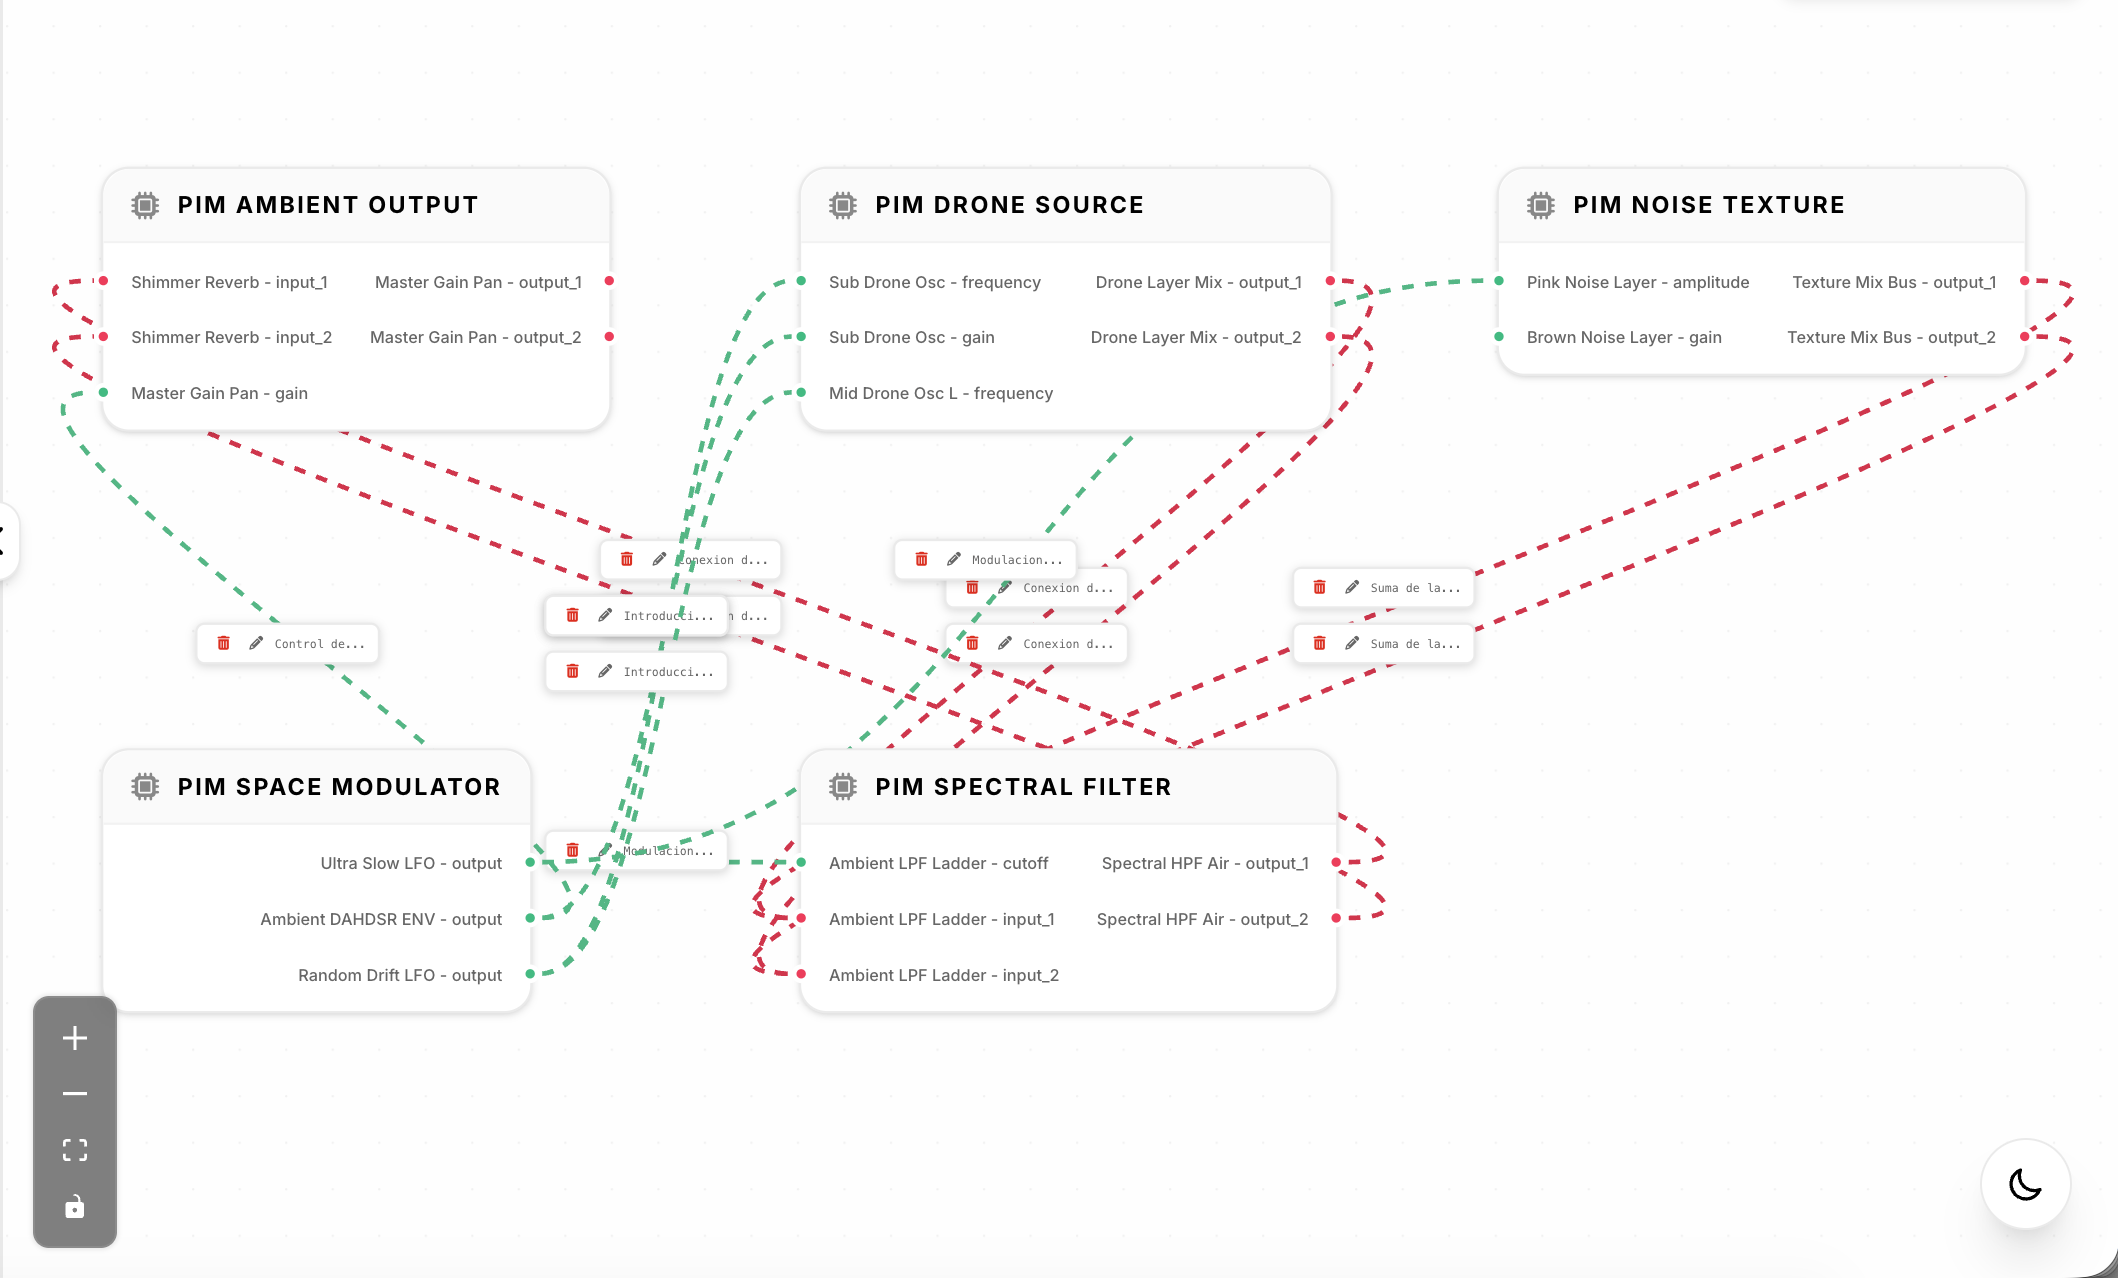
\includegraphics[width=\textwidth]{imagenes/06_diseno/05_visorGraficoRelacionesPim.png}
    \caption{Visor gráfico de la red de relaciones PIM.}
\end{figure}

El grafo de \textit{PIM} revela la complejidad de la arquitectura diseñada. A diferencia del \textit{CIM}, las conexiones en esta fase suelen representar flujos de datos de audio concretos, señales de control y eventos del sistema.

\begin{figure}[!ht]
    \centering
    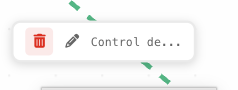
\includegraphics[width=0.5\textwidth]{imagenes/06_diseno/06_edicionGraficasAristasPim.png}
    \caption{Controles contextuales para la edición de aristas en el visor gráfico.}
\end{figure}

\begin{figure}[!ht]
    \centering
    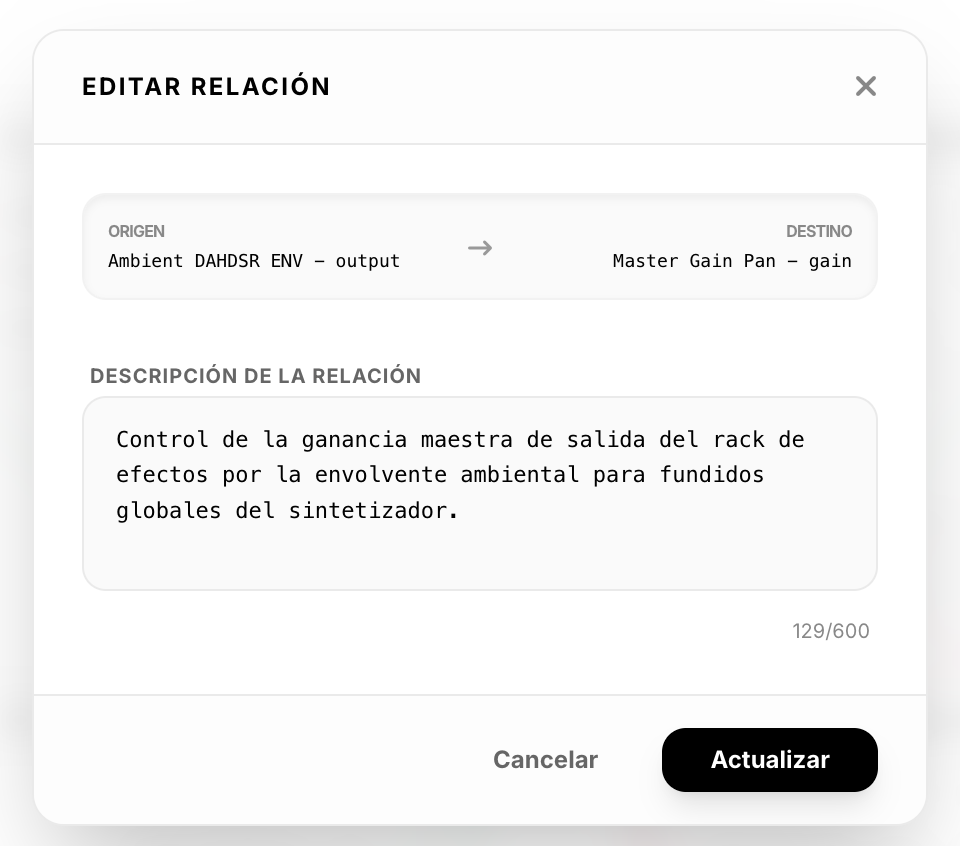
\includegraphics[width=0.6\textwidth]{imagenes/06_diseno/07_formularioEdicionGraficoAristasPim.png}
    \caption{Formulario rápido para ajustar la configuración de una conexión.}
\end{figure}

El entorno gráfico no es solo de consulta. Integrados en los elementos visuales, se encuentran controles que permiten editar directamente las propiedades de las aristas (como asignar tipos de puerto o alterar cardinalidades) sin necesidad de recurrir al código.

\begin{figure}[!ht]
    \centering
    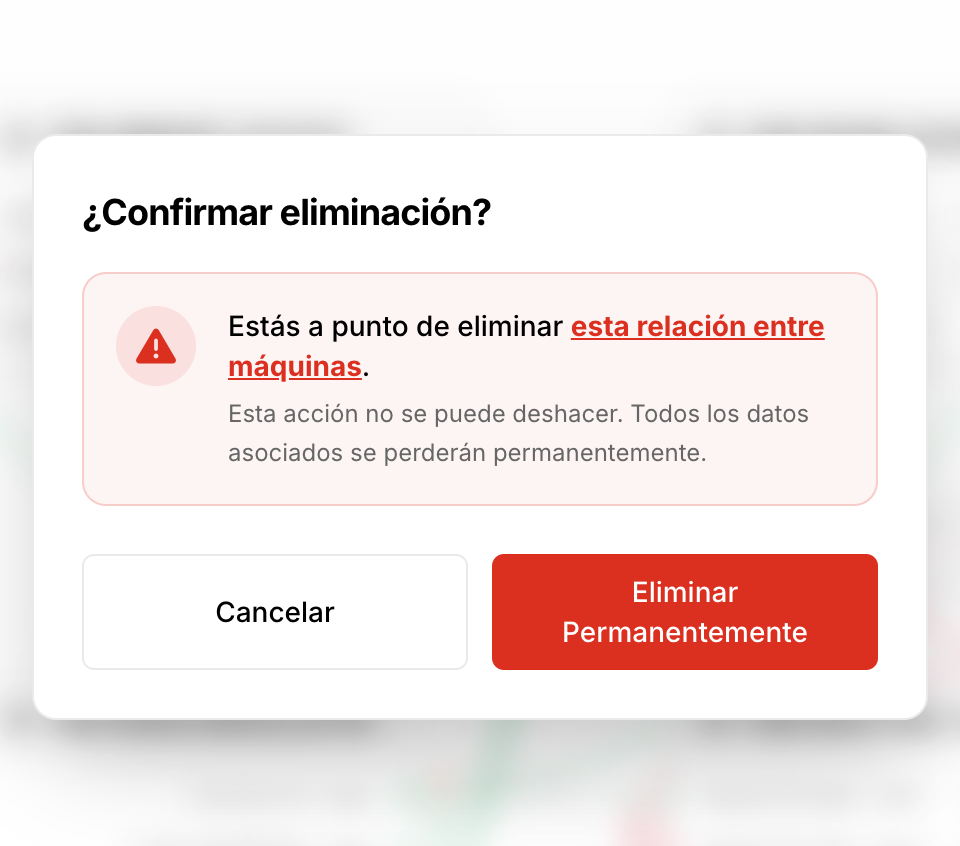
\includegraphics[width=0.6\textwidth]{imagenes/06_diseno/08_eliminarGraficamenteAristaPim.png}
    \caption{Confirmación al eliminar una arista directamente desde el entorno gráfico.}
\end{figure}

La topología puede ser modificada interactivamente, incluyendo la eliminación de enlaces, siempre mediada por ventanas de confirmación para evitar acciones destructivas accidentales.

\subsection{Edición mediante Código JSON}

\begin{figure}[!ht]
    \centering
    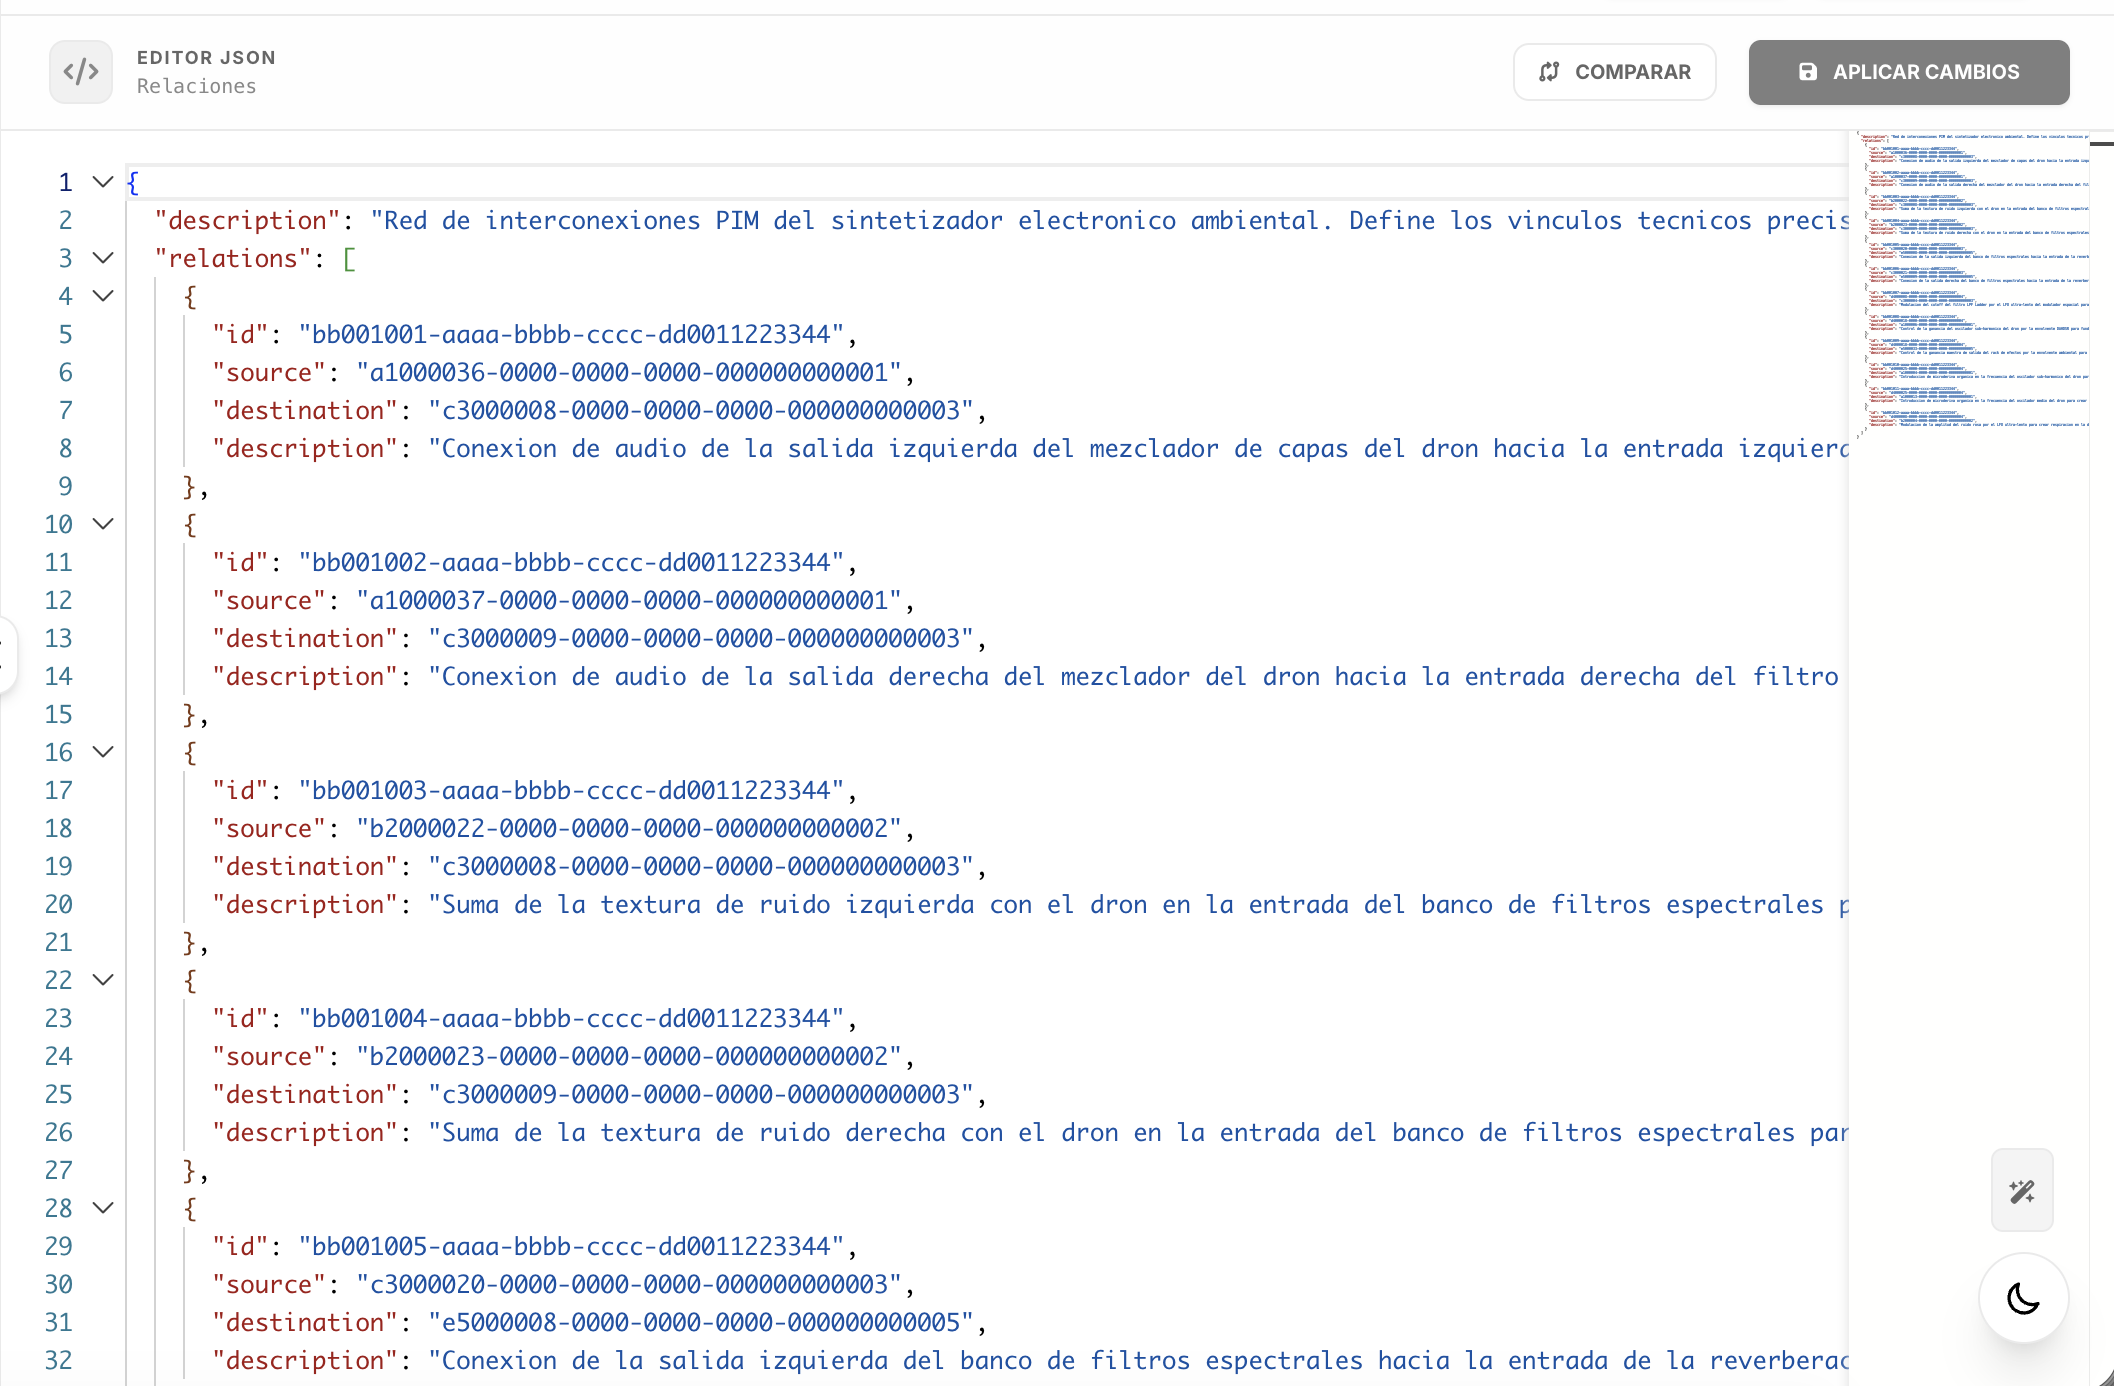
\includegraphics[width=\textwidth]{imagenes/06_diseno/09_edicionJsonRelacionesPim.png}
    \caption{Editor de código JSON para relaciones PIM.}
\end{figure}

Para manipulaciones granulares y ajustes de la estructura \textit{DSL}, se dispone del editor \textit{JSON} enfocado al modelo \textit{PIM}.

\begin{figure}[!ht]
    \centering
    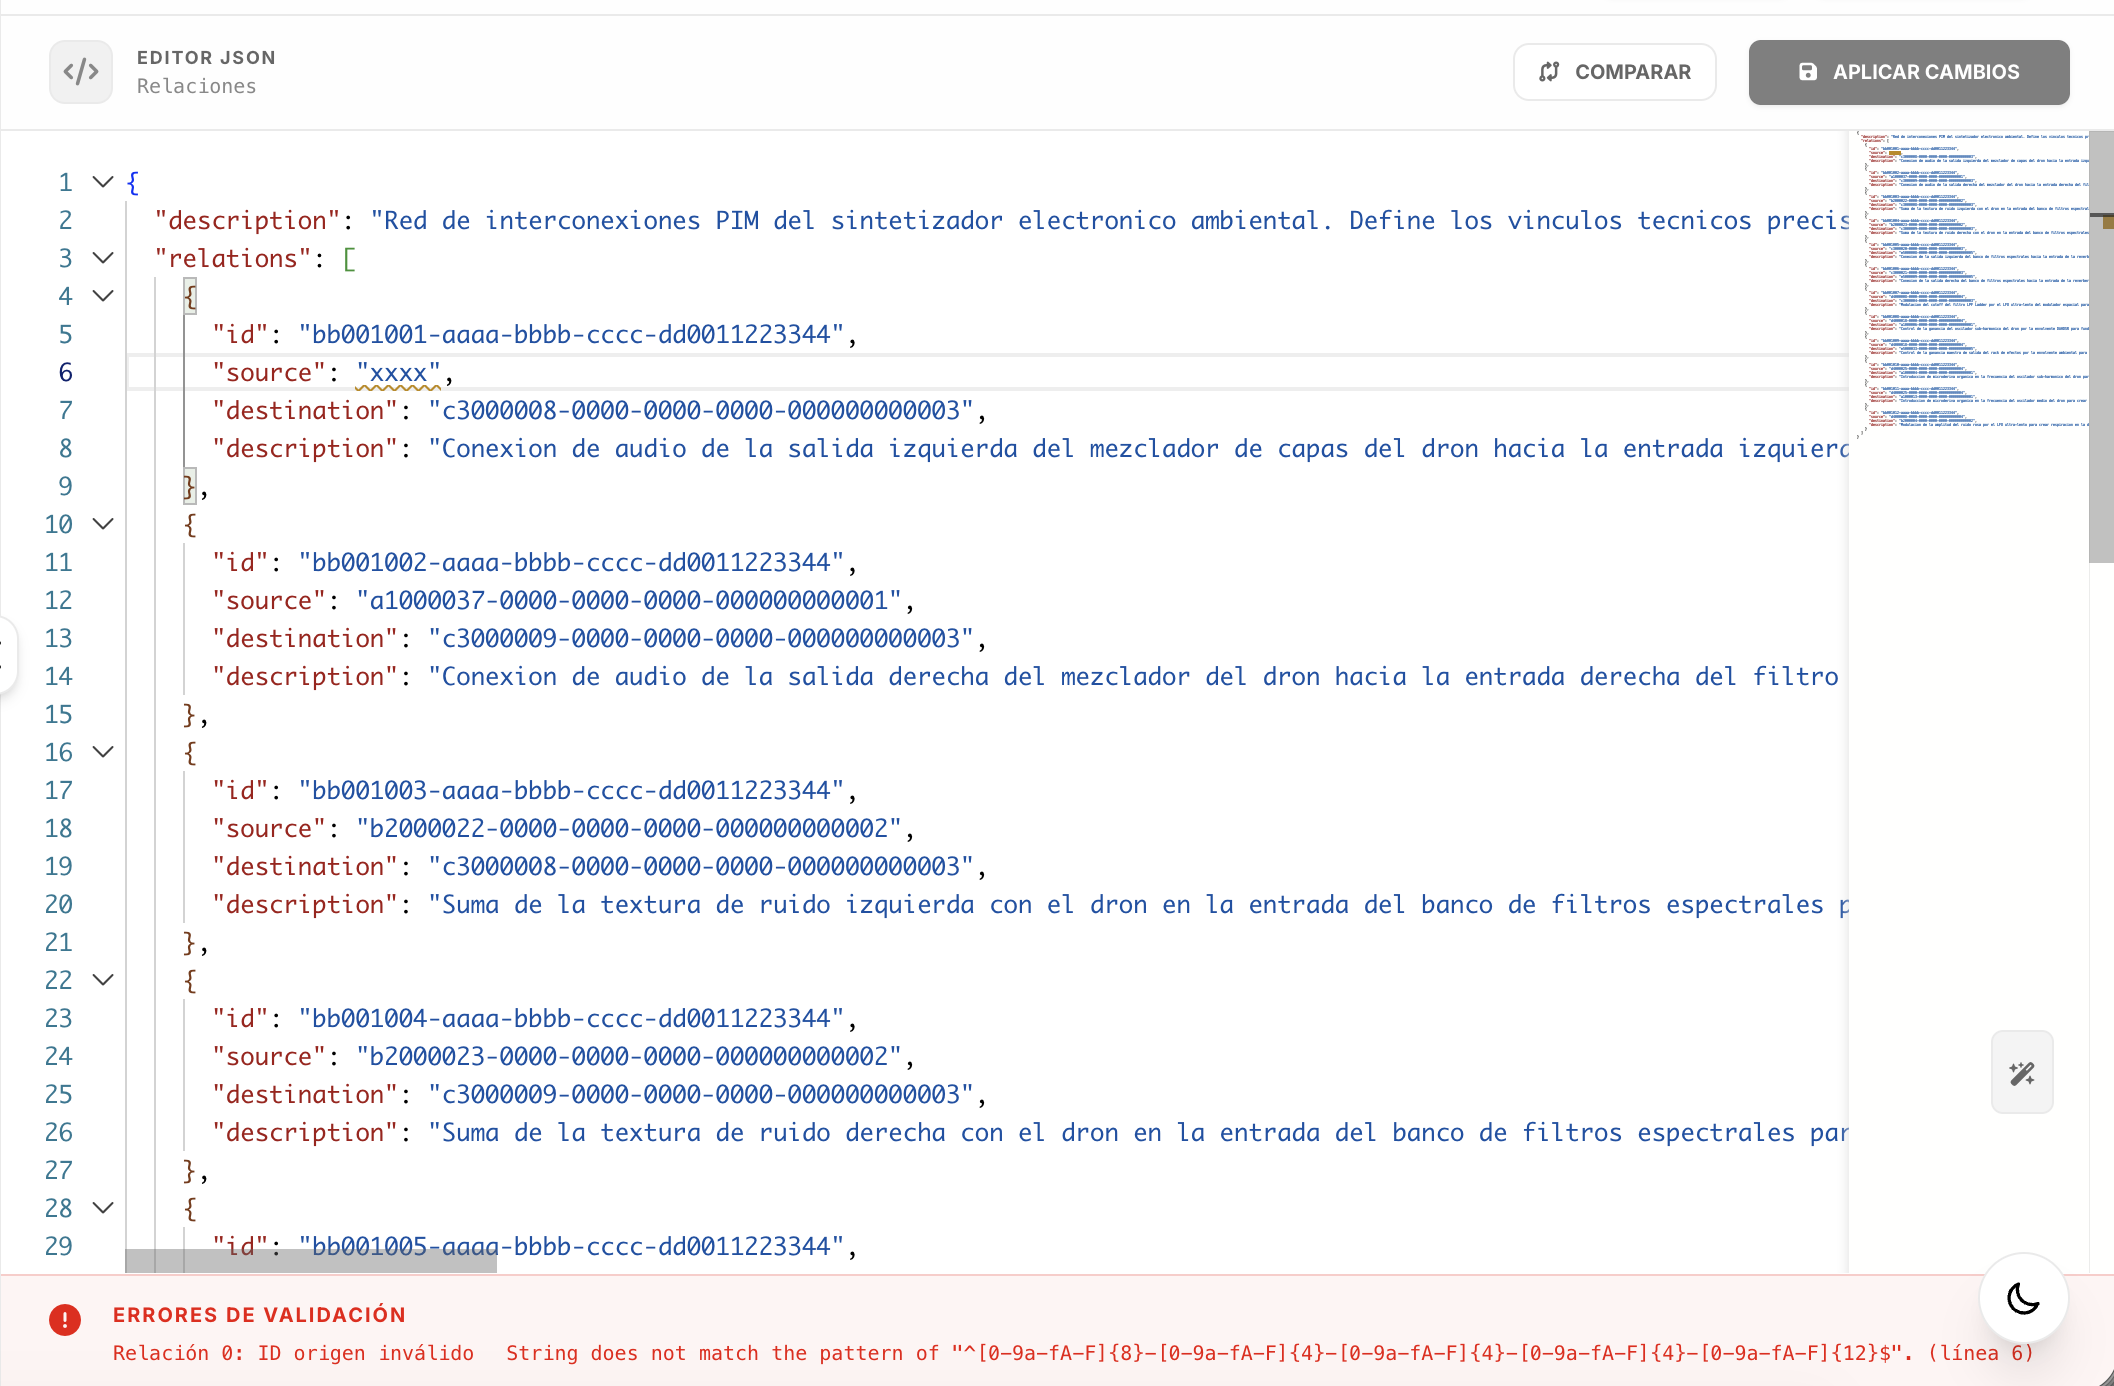
\includegraphics[width=\textwidth]{imagenes/06_diseno/10_edicionJsonRelacionesPimValidacion.png}
    \caption{Validación de esquema y reglas de diseño en el editor JSON.}
\end{figure}

Este editor incorpora capacidades de validación estrictas, verificando que el código cumple con las normativas del metamodelo \textit{PIM}, resaltando cualquier inconsistencia estructural antes de su almacenamiento.

\begin{figure}[!ht]
    \centering
    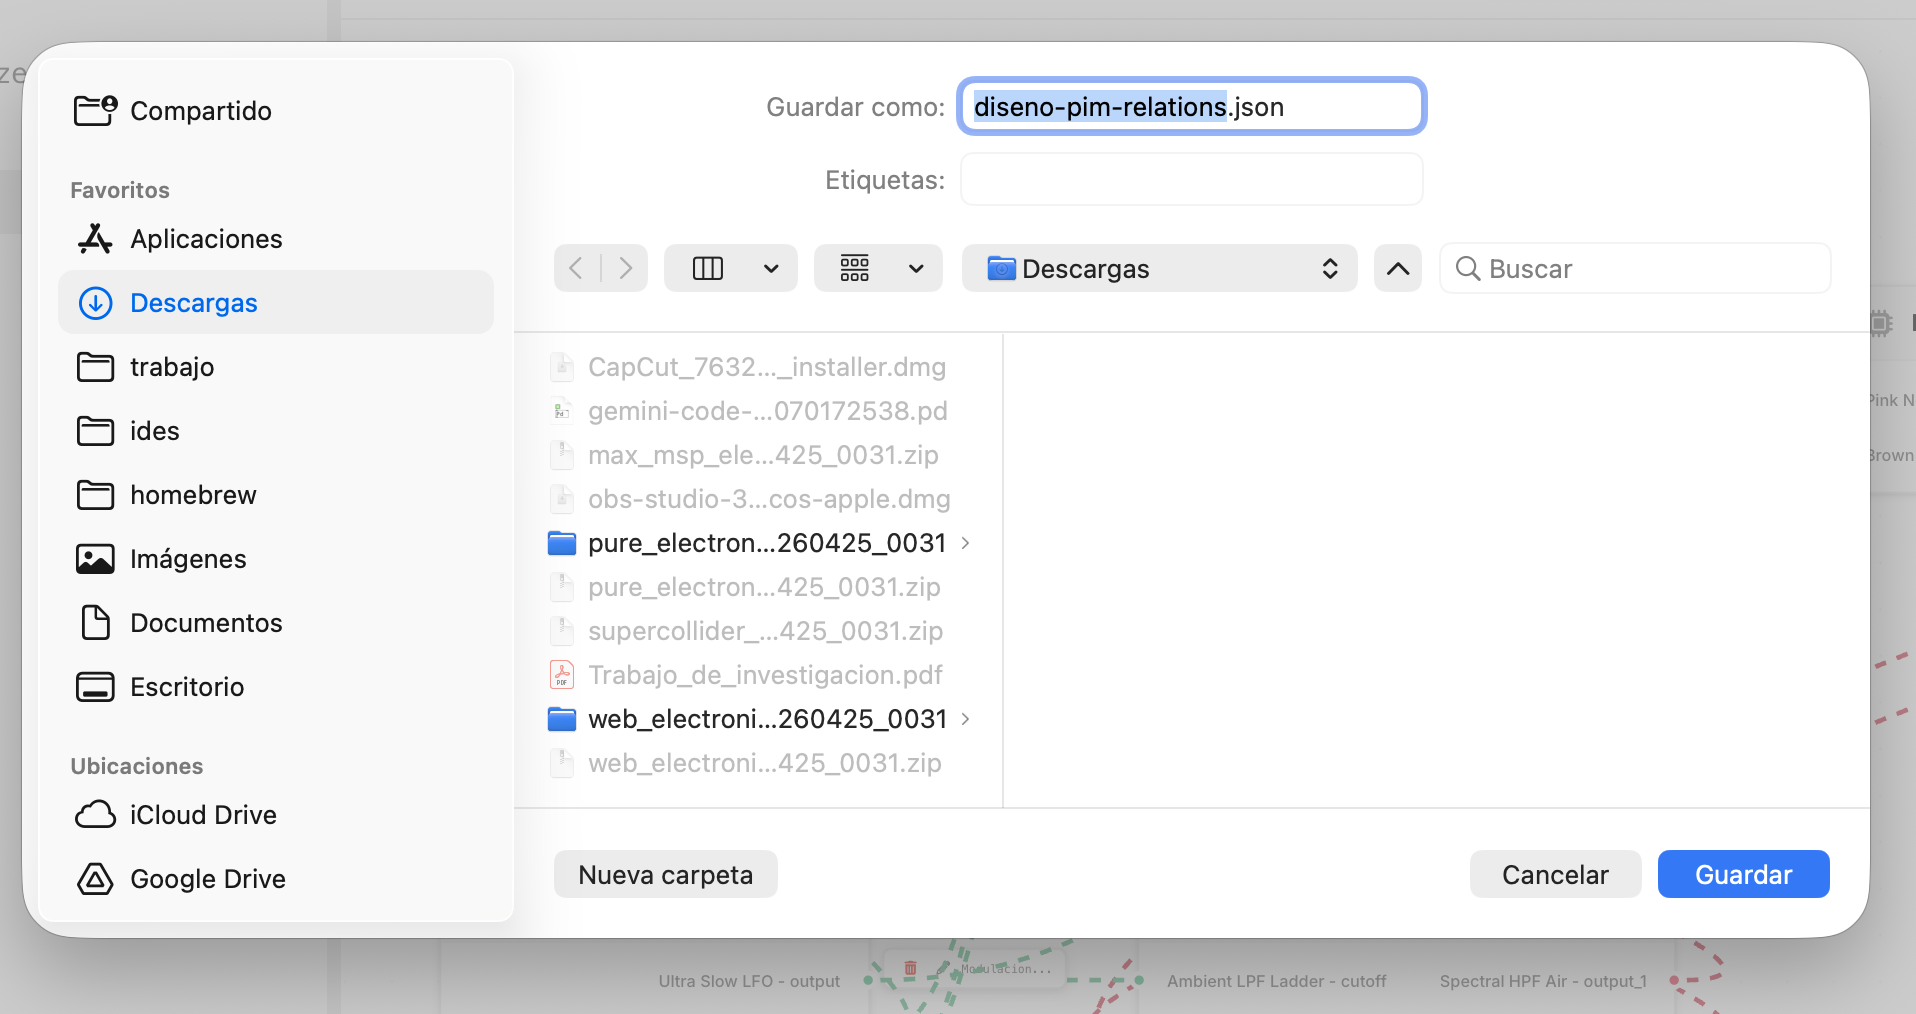
\includegraphics[width=0.6\textwidth]{imagenes/06_diseno/11_exportarJsonRelacionesPim.png}
    \caption{Opción para exportar el modelo PIM a nivel de relaciones.}
\end{figure}

\begin{figure}[!ht]
    \centering
    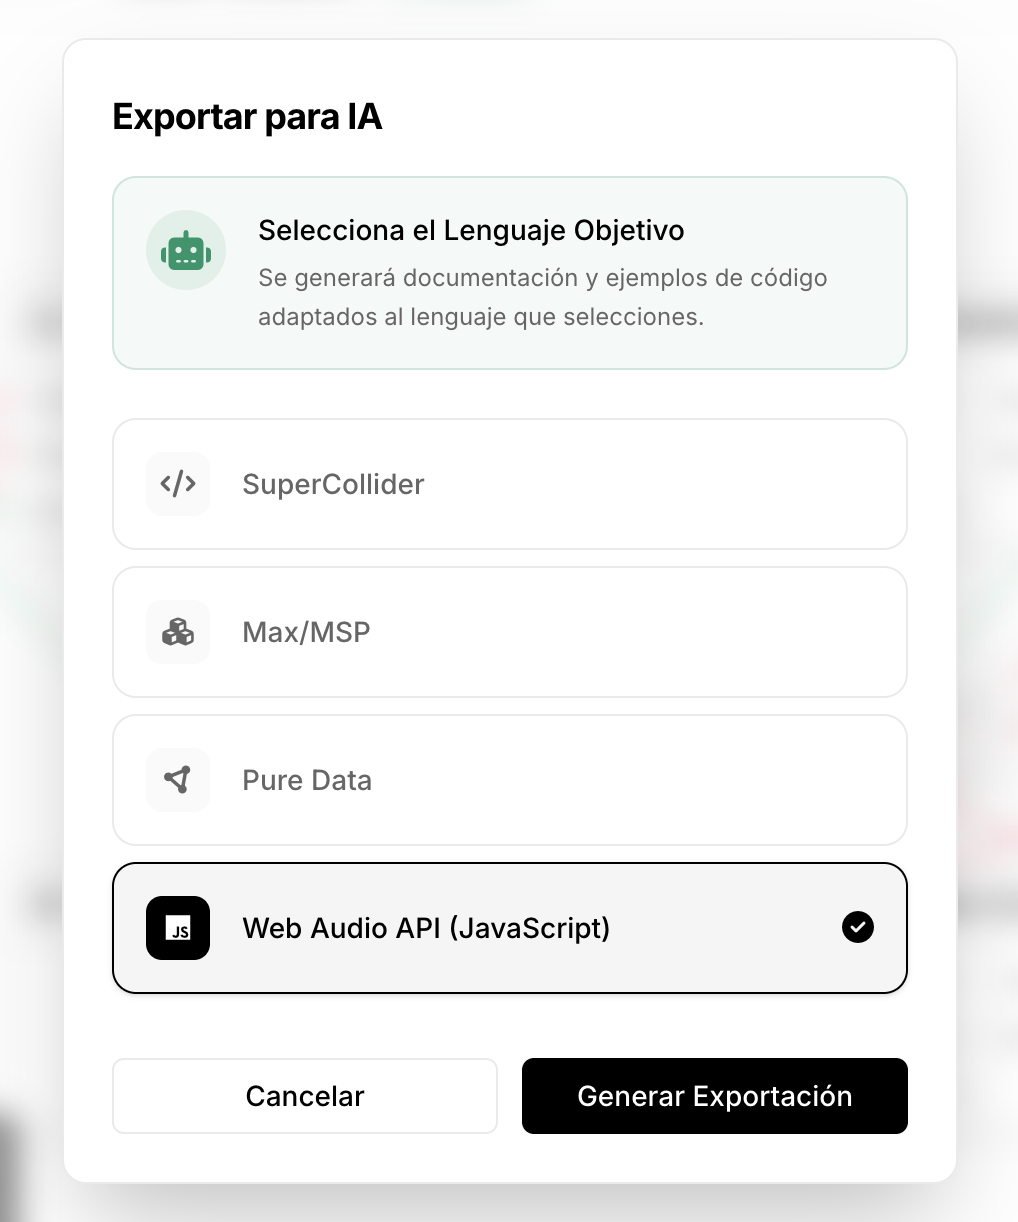
\includegraphics[width=0.4\textwidth]{imagenes/06_diseno/12_exportarParaIA.png}
    \caption{Opción de exportación de contexto para Inteligencia Artificial.}
\end{figure}

Junto a la exportación estándar del fichero \textit{JSON}, el nivel \textit{PIM} habilita utilidades avanzadas como la ``Exportación para IA'', diseñada para extraer el contexto del proyecto y facilitar la asistencia de herramientas generativas externas.

\section{Configuración de Máquinas PIM}

\begin{figure}[!ht]
    \centering
    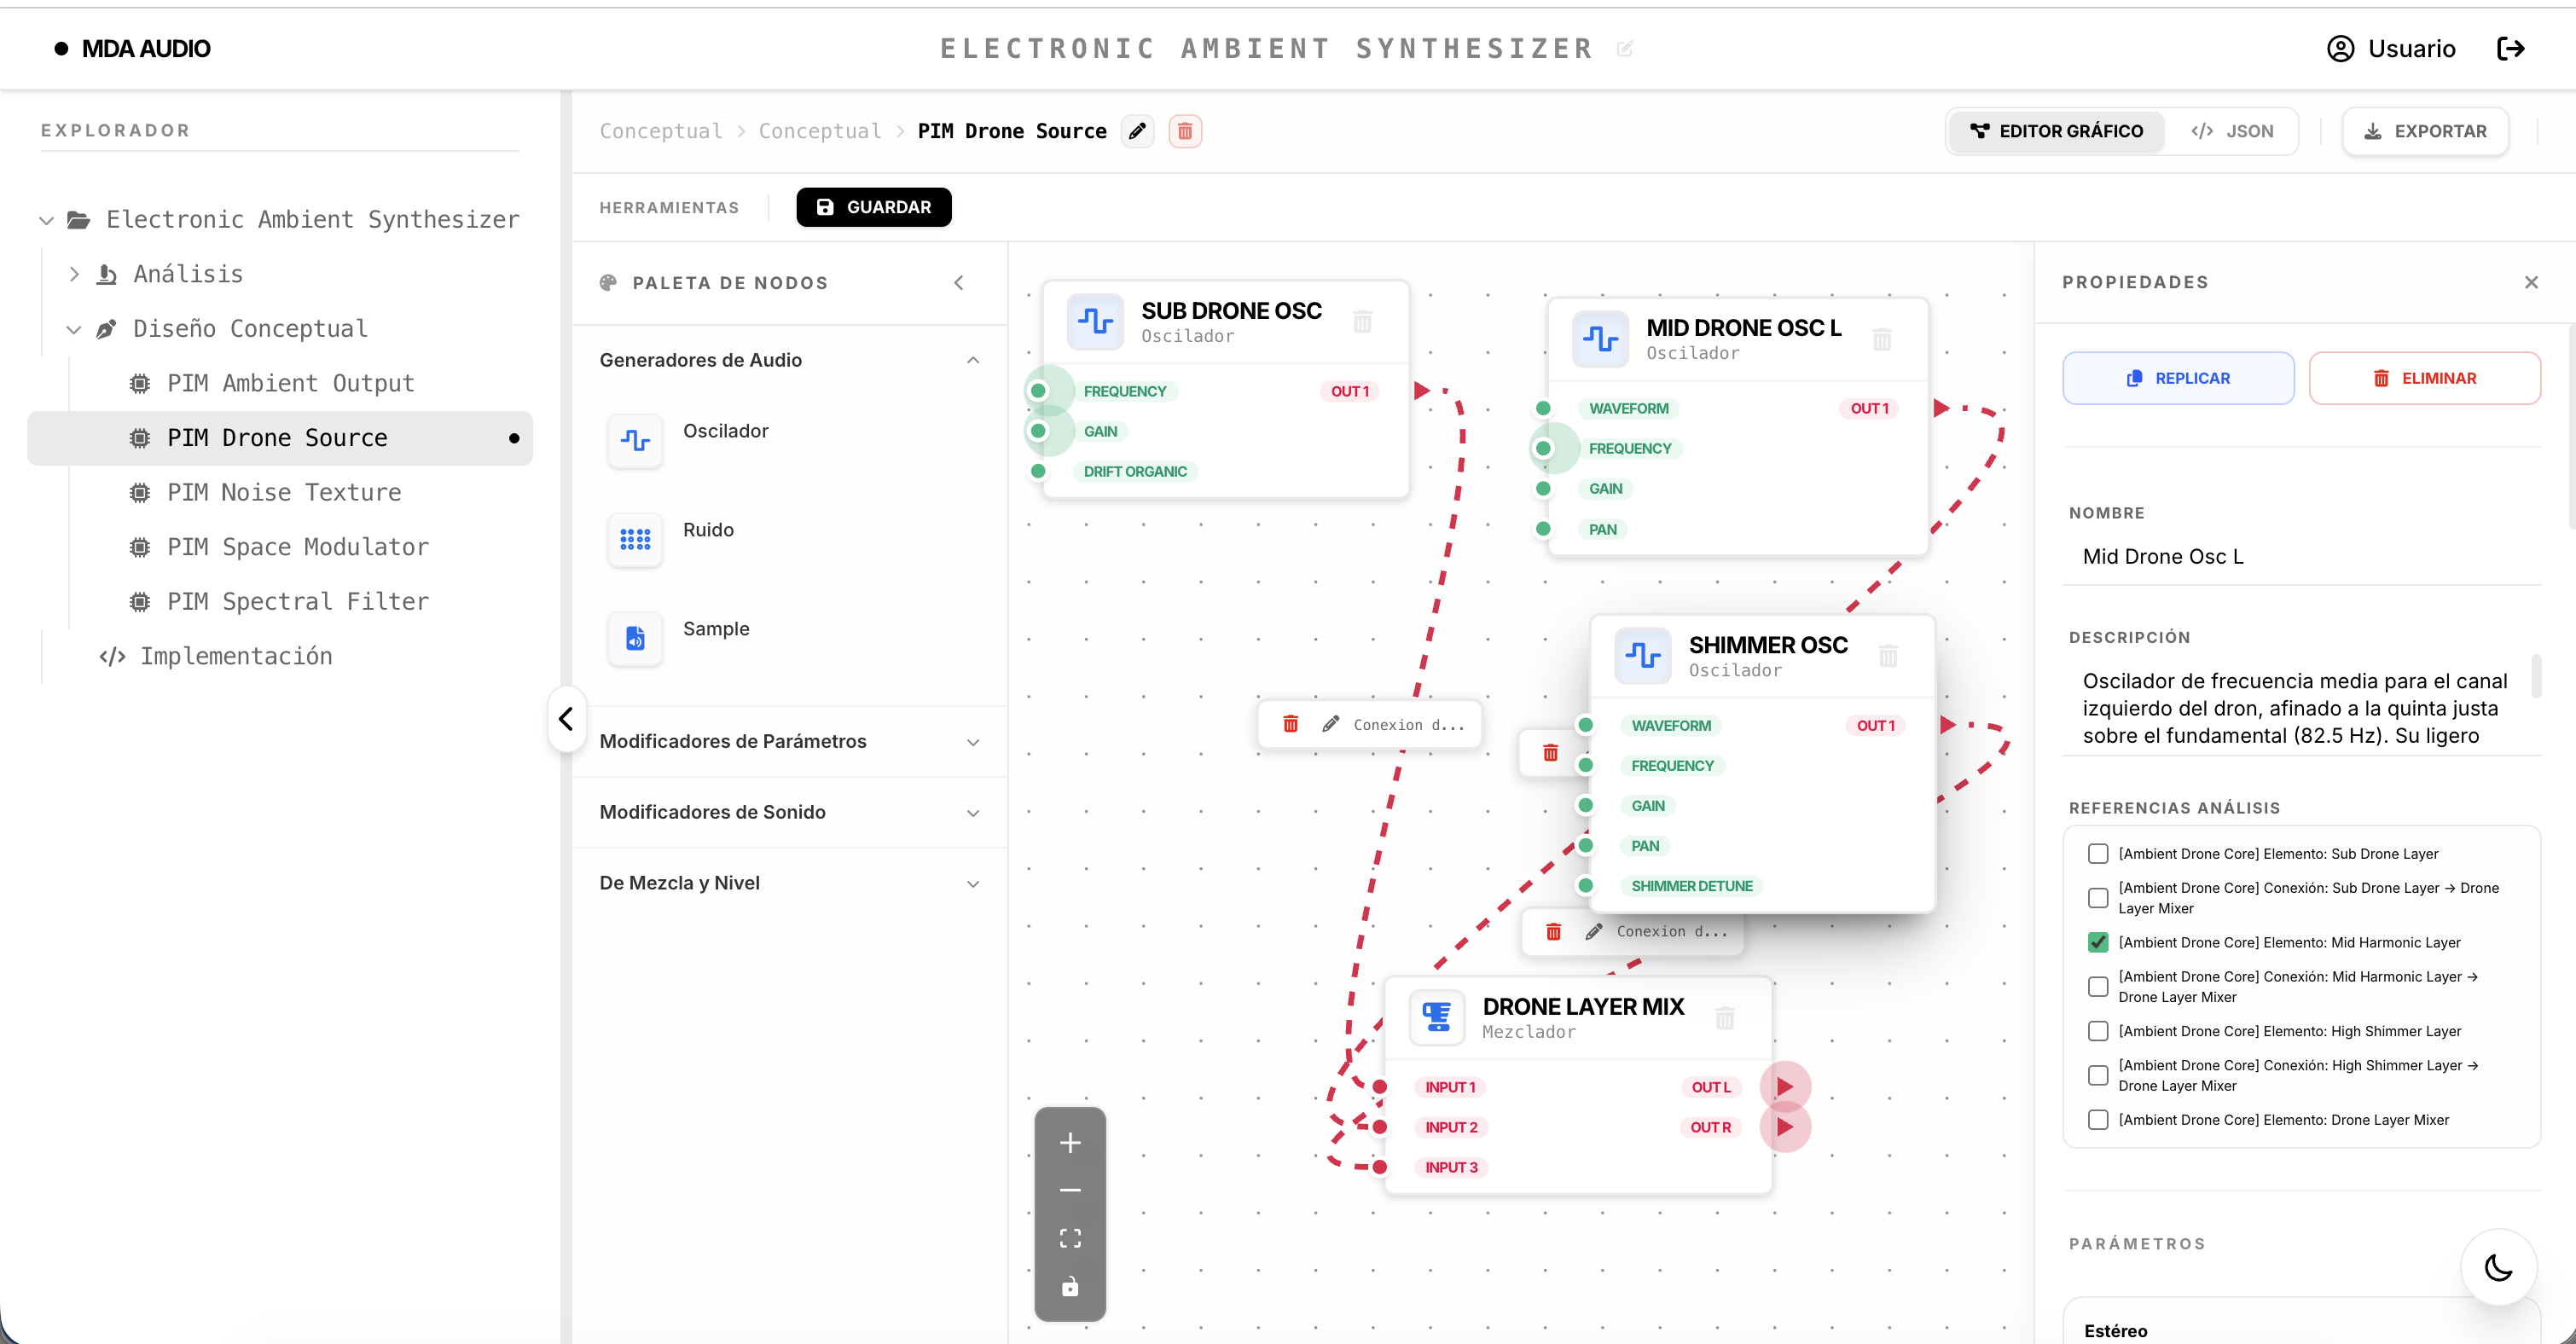
\includegraphics[width=\textwidth]{imagenes/06_diseno/13_pantallaMaquinaPim.png}
    \caption{Pantalla de detalle para la configuración de una máquina PIM específica.}
\end{figure}

Seleccionando una máquina desde el explorador bajo la rama \textit{PIM}, se accede a su entorno de configuración detallada.

\begin{figure}[!ht]
    \centering
    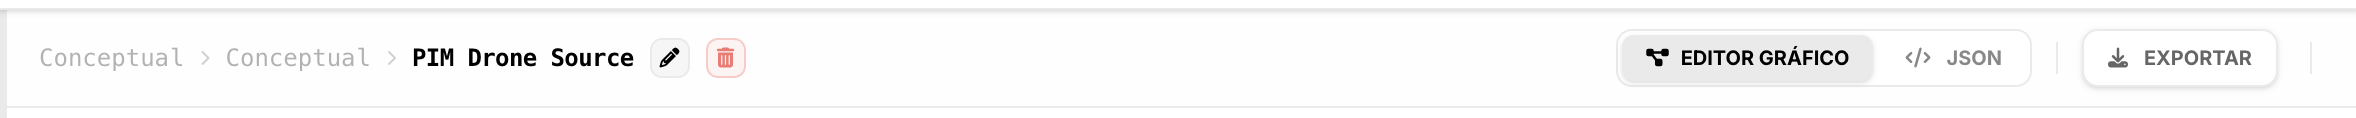
\includegraphics[width=\textwidth]{imagenes/06_diseno/14_barraMaquinaPim.png}
    \caption{Barra de herramientas contextual para la gestión de la máquina PIM.}
\end{figure}

\begin{figure}[!ht]
    \centering
    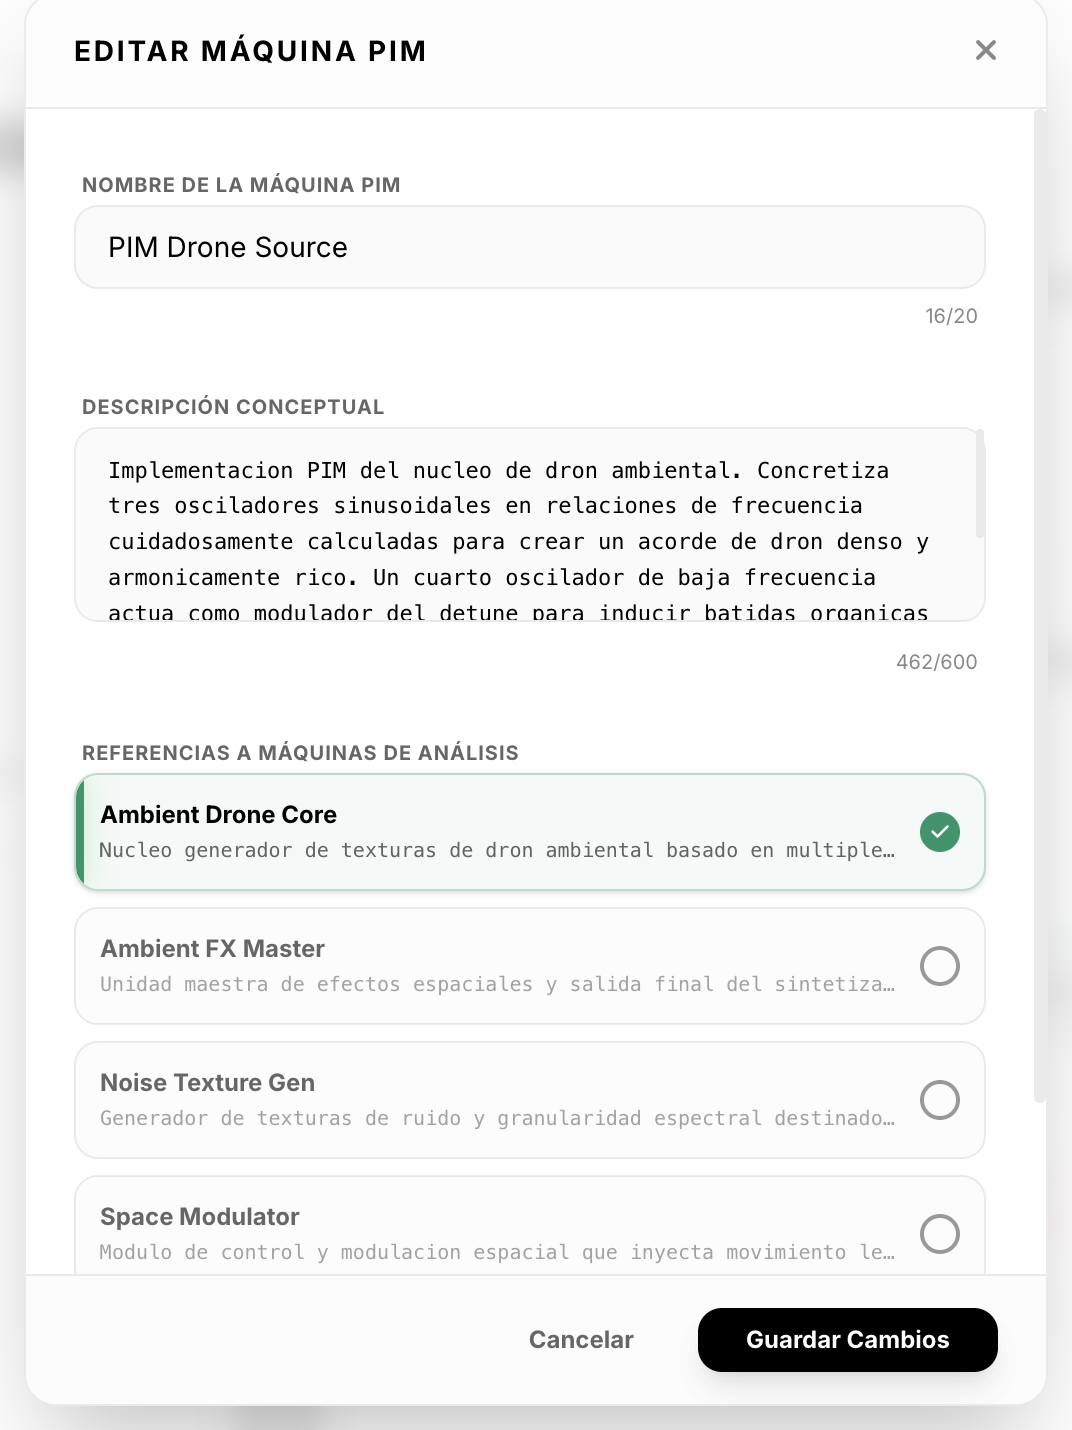
\includegraphics[width=0.6\textwidth]{imagenes/06_diseno/15_editarMaquinaPim.png}
    \caption{Formulario para modificar las propiedades principales de la máquina.}
\end{figure}

La barra de herramientas de la máquina permite acceder rápidamente a su edición, posibilitando ajustar su identificador o actualizar sus referencias a elementos del modelo \textit{CIM}.

\begin{figure}[!ht]
    \centering
    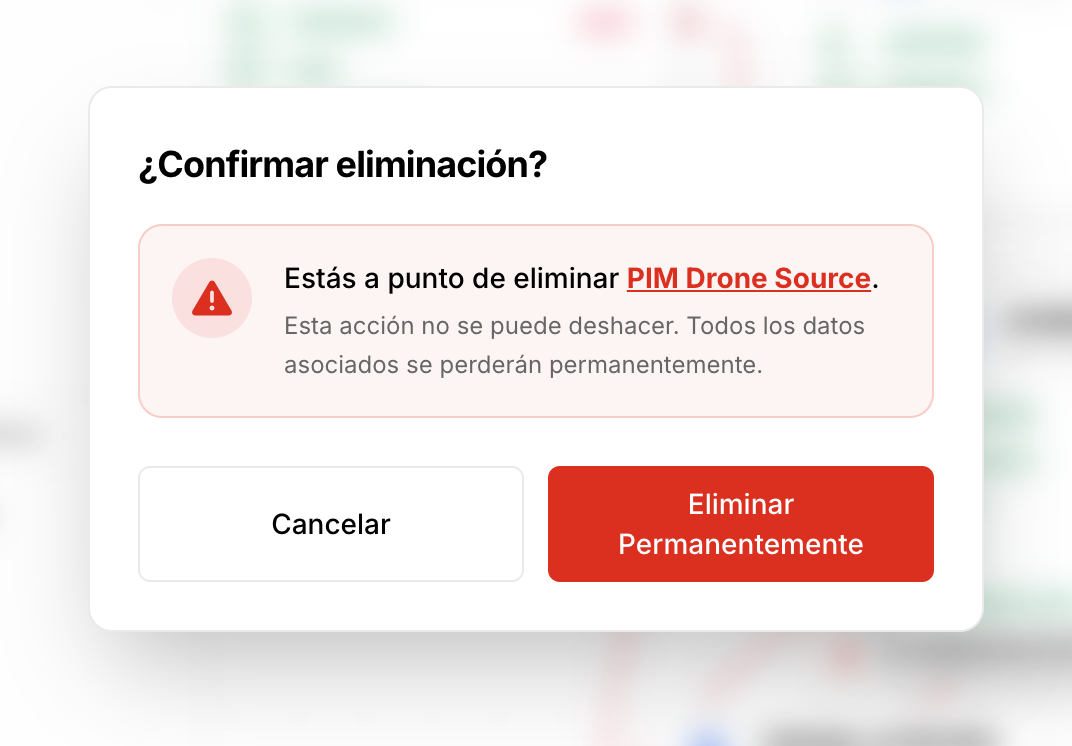
\includegraphics[width=0.6\textwidth]{imagenes/06_diseno/16_eliminarMaquinaPim.png}
    \caption{Proceso de eliminación segura de una máquina PIM.}
\end{figure}

Si la máquina ya no es necesaria en el diseño, se puede eliminar mediante la correspondiente validación de seguridad.

\subsection{Validación y Control de Versiones Interno}

\begin{figure}[!ht]
    \centering
    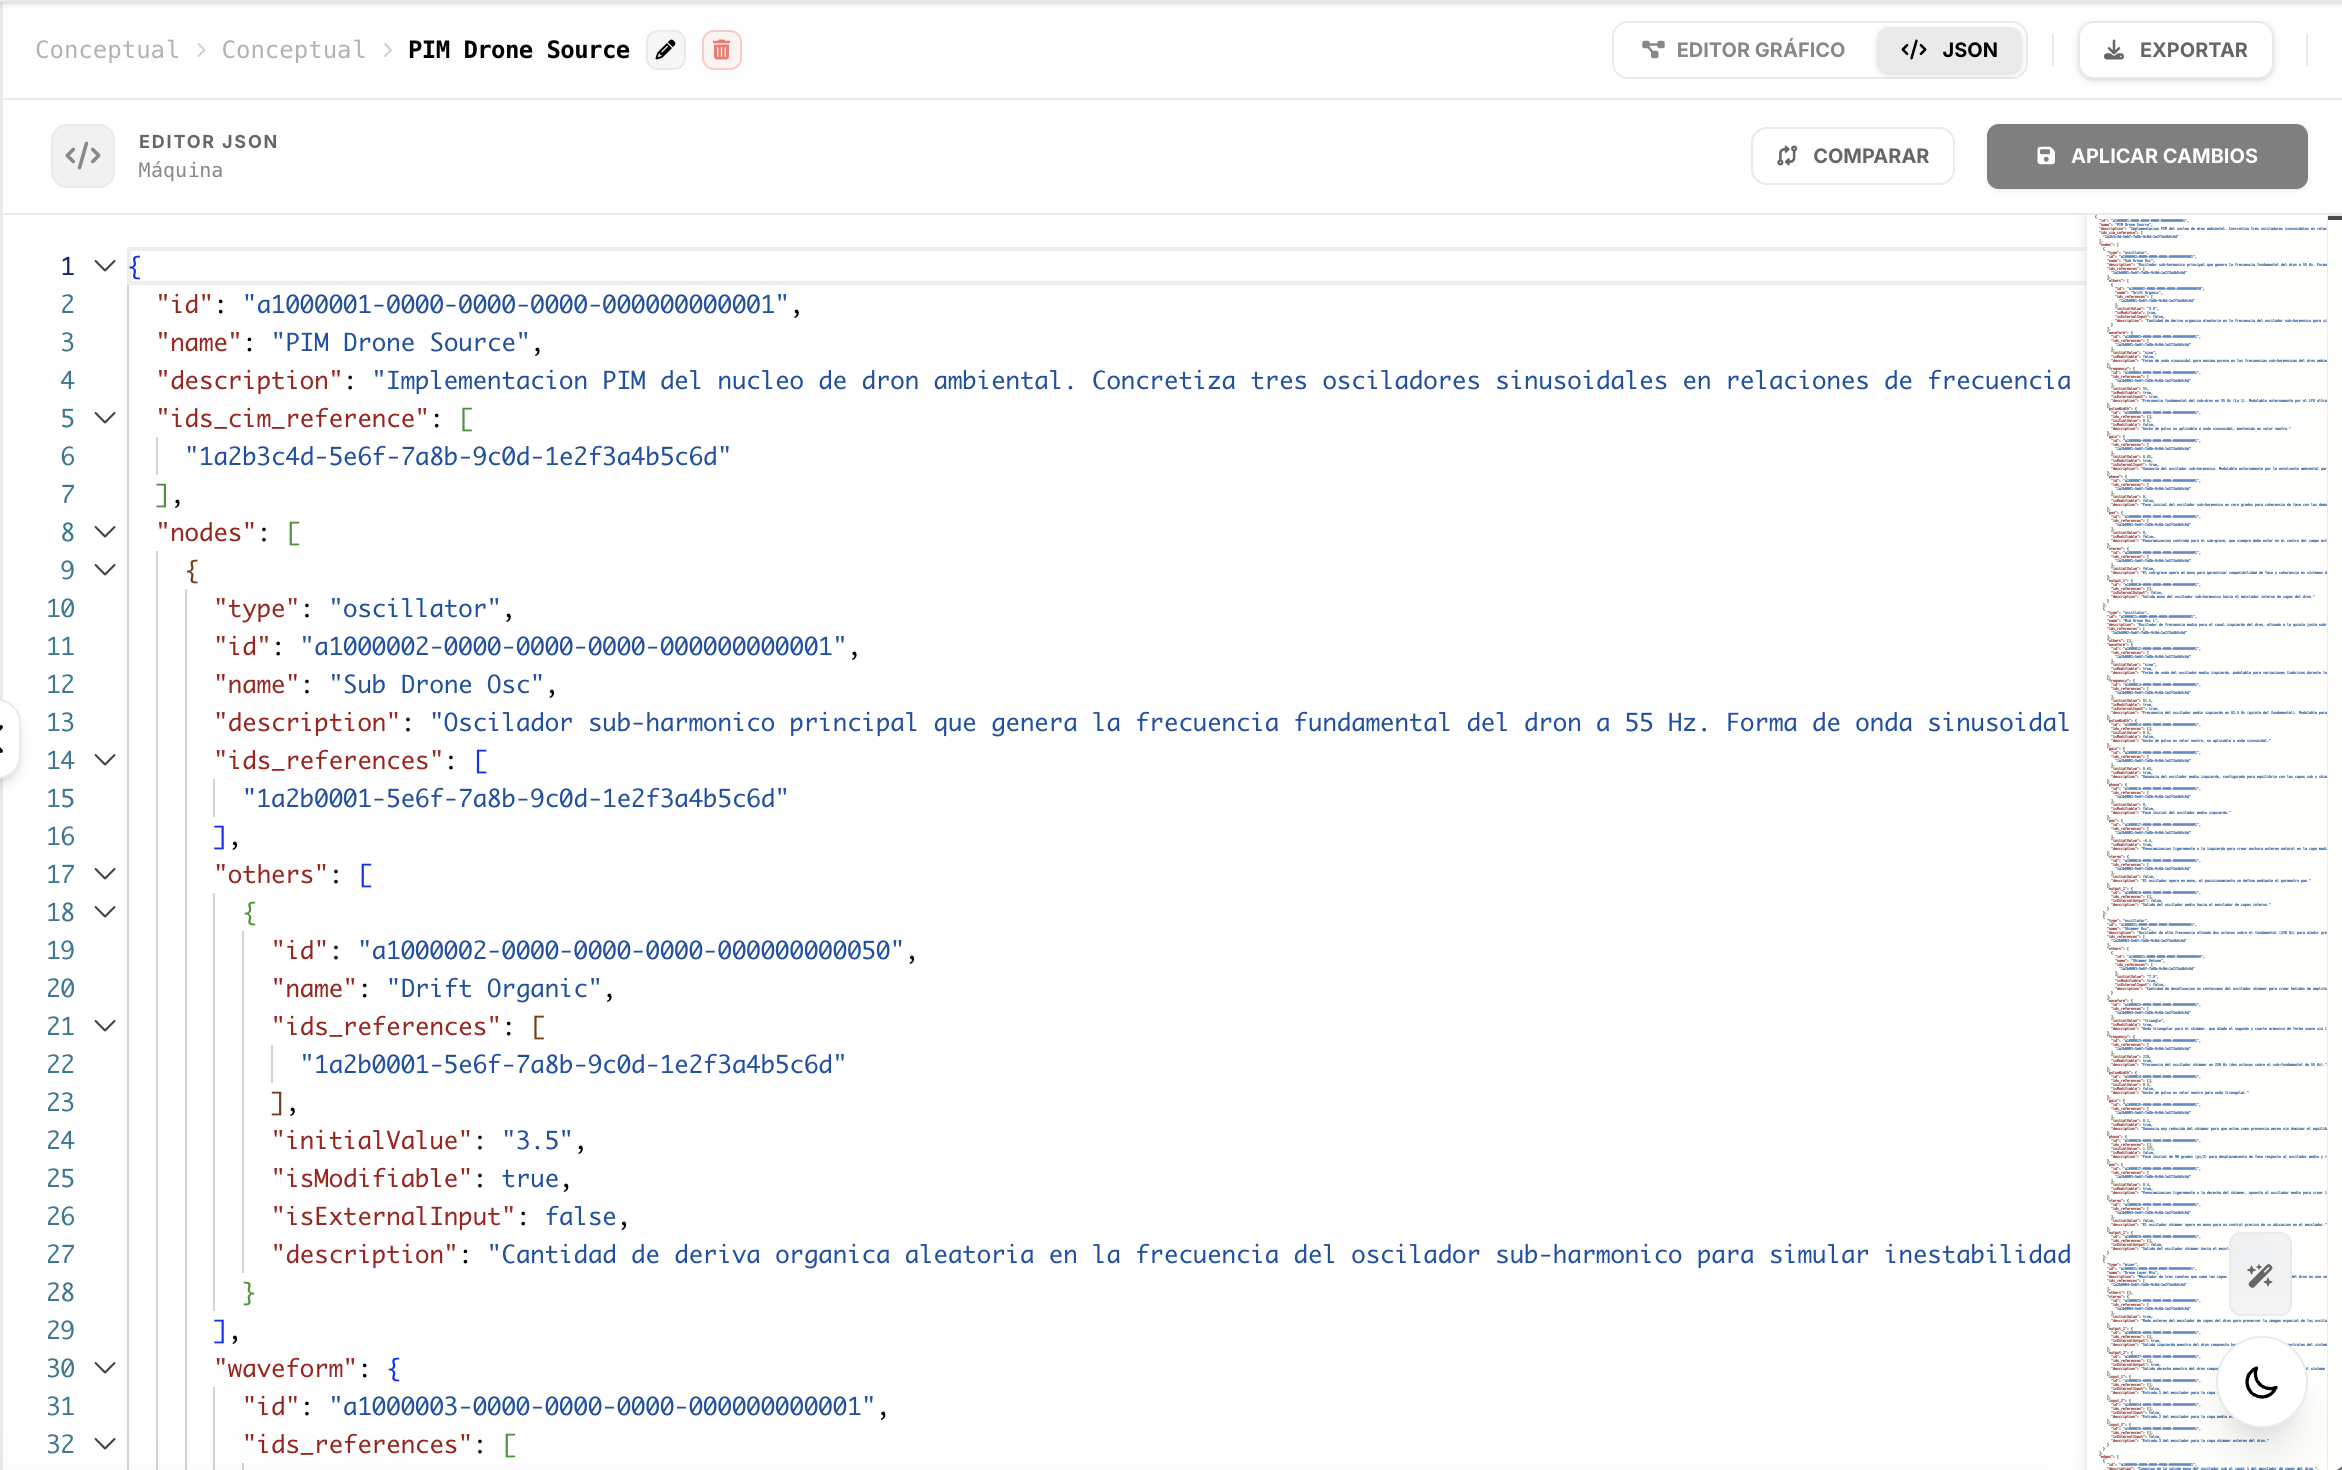
\includegraphics[width=\textwidth]{imagenes/06_diseno/17_edicionJsonMaquinaPim.png}
    \caption{Editor de código de la definición interna de la máquina PIM.}
\end{figure}

\begin{figure}[!ht]
    \centering
    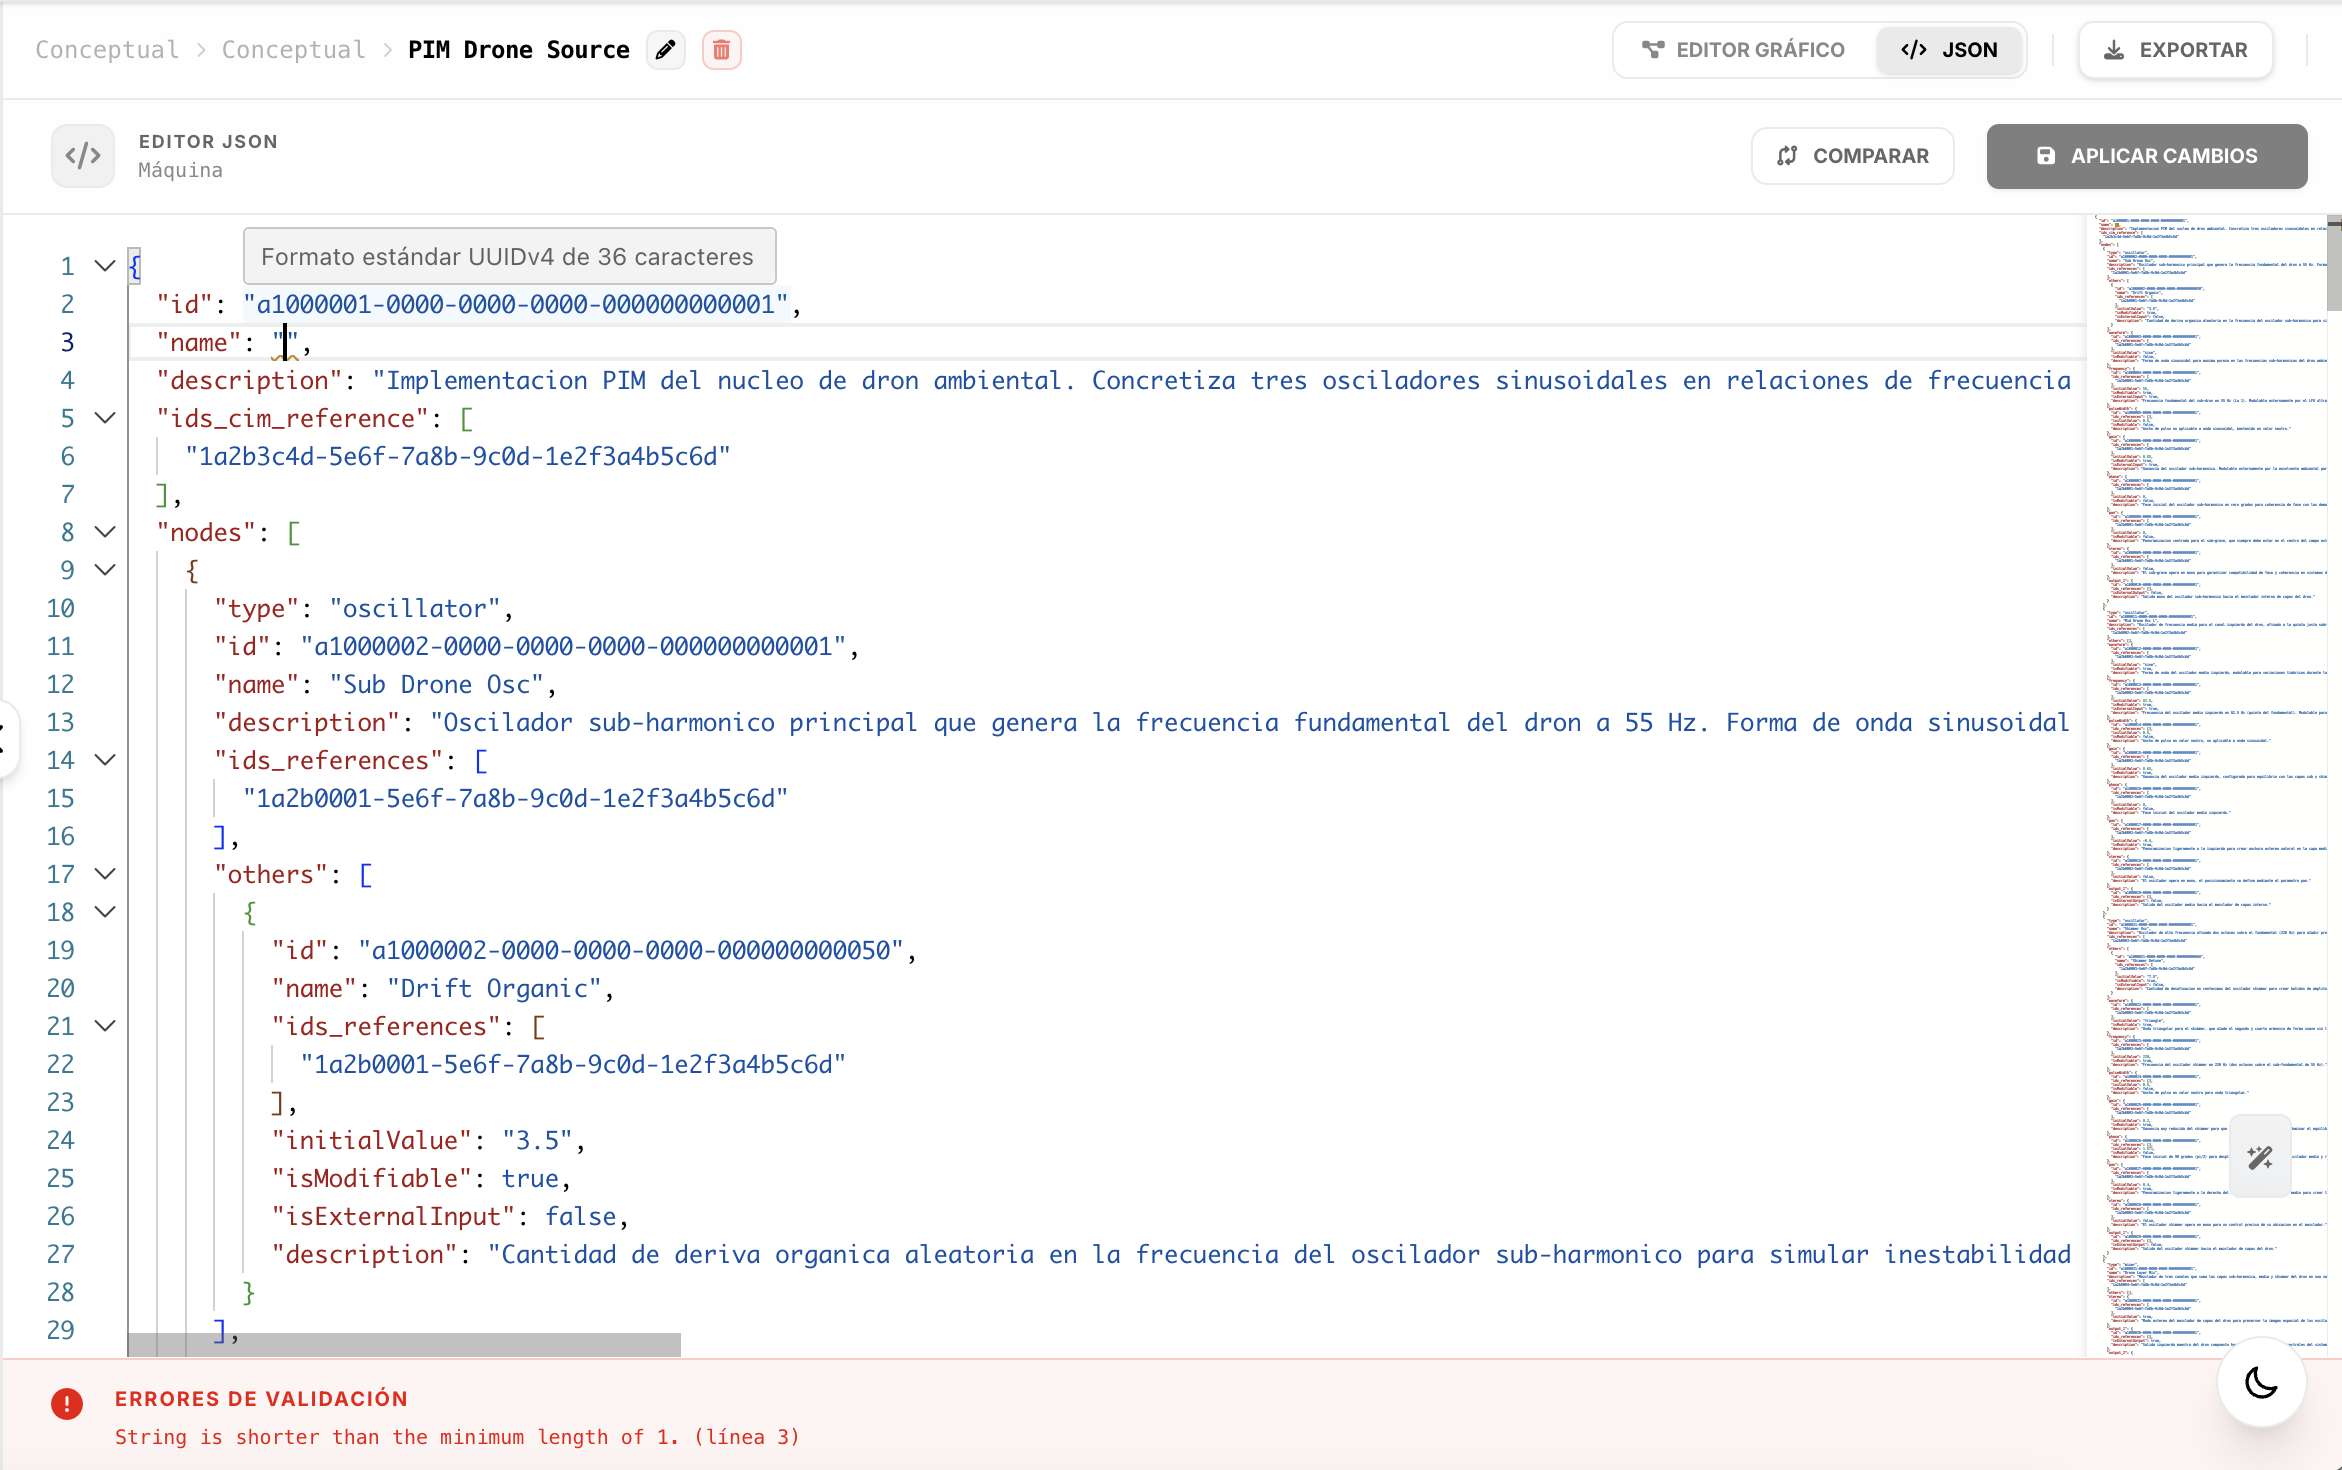
\includegraphics[width=\textwidth]{imagenes/06_diseno/18_edicionJsonMaquinaPimValidacion.png}
    \caption{Detección de errores y comprobación de integridad en la máquina PIM.}
\end{figure}

El modelado profundo de la máquina se realiza mediante su editor de código. Las reglas del dominio validan la consistencia de los bloques lógicos de síntesis, señalando errores sintácticos o discrepancias con las definiciones conceptuales.

\begin{figure}[!ht]
    \centering
    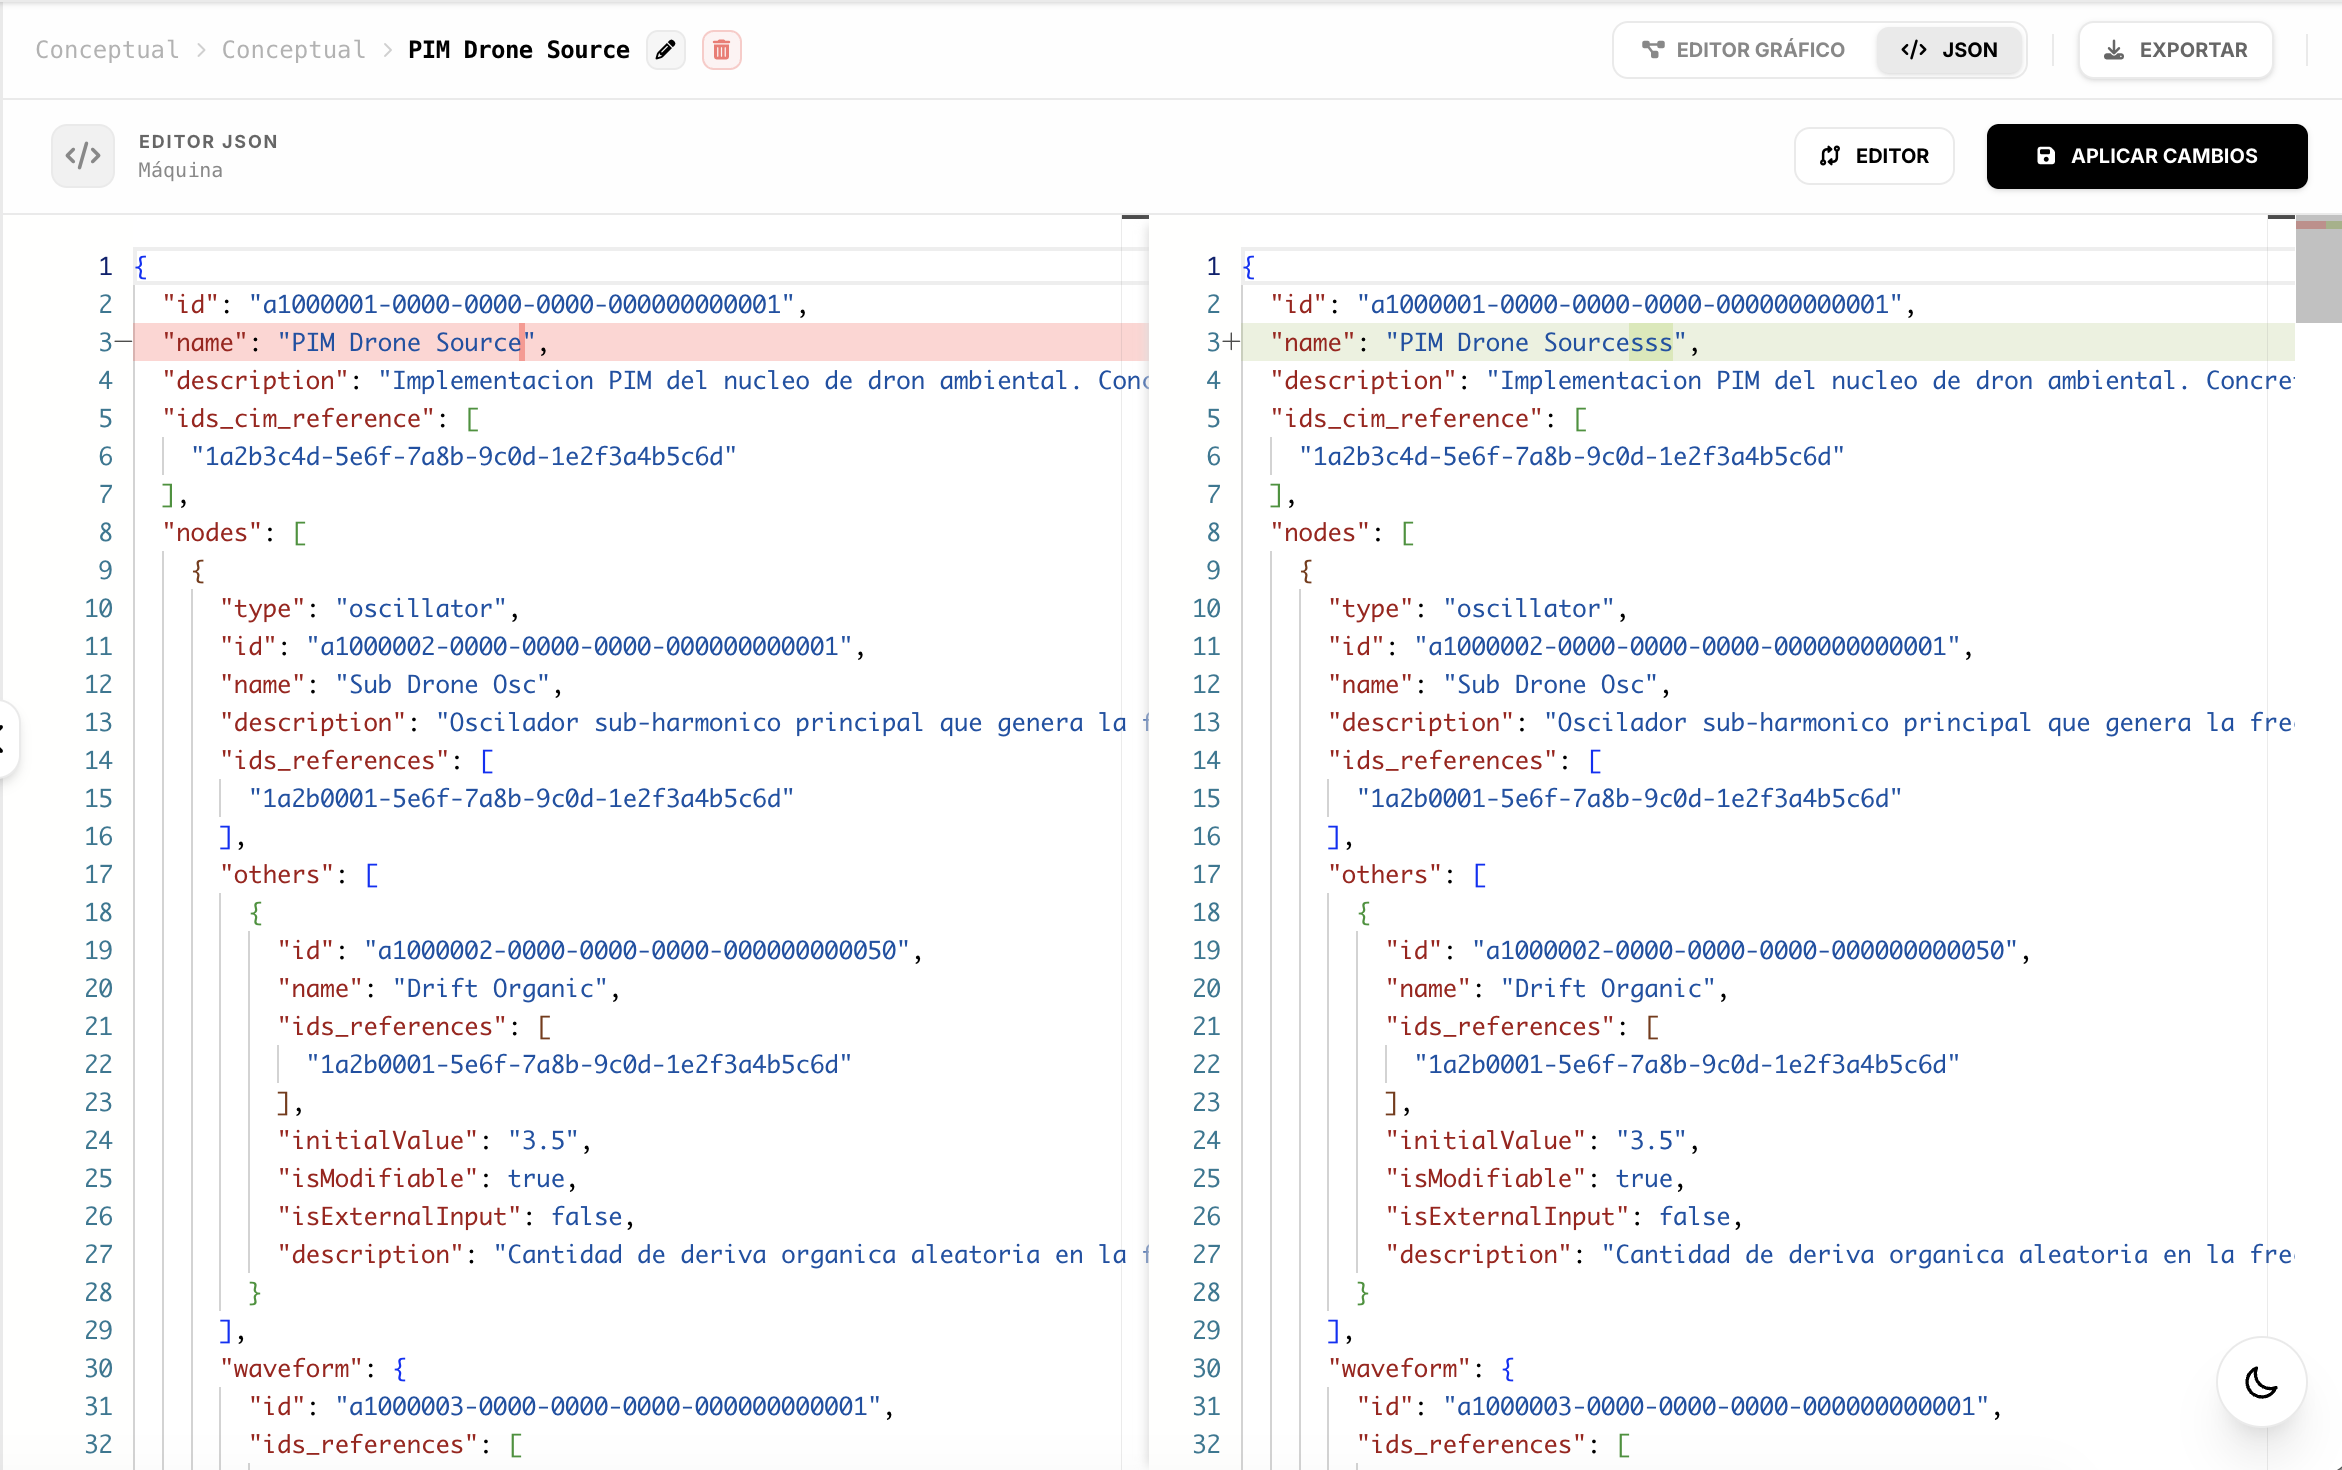
\includegraphics[width=\textwidth]{imagenes/06_diseno/19_edicionJsonMaquinaPimComparacion.png}
    \caption{Uso de la herramienta Diff para auditar cambios en la configuración interna.}
\end{figure}

\begin{figure}[!ht]
    \centering
    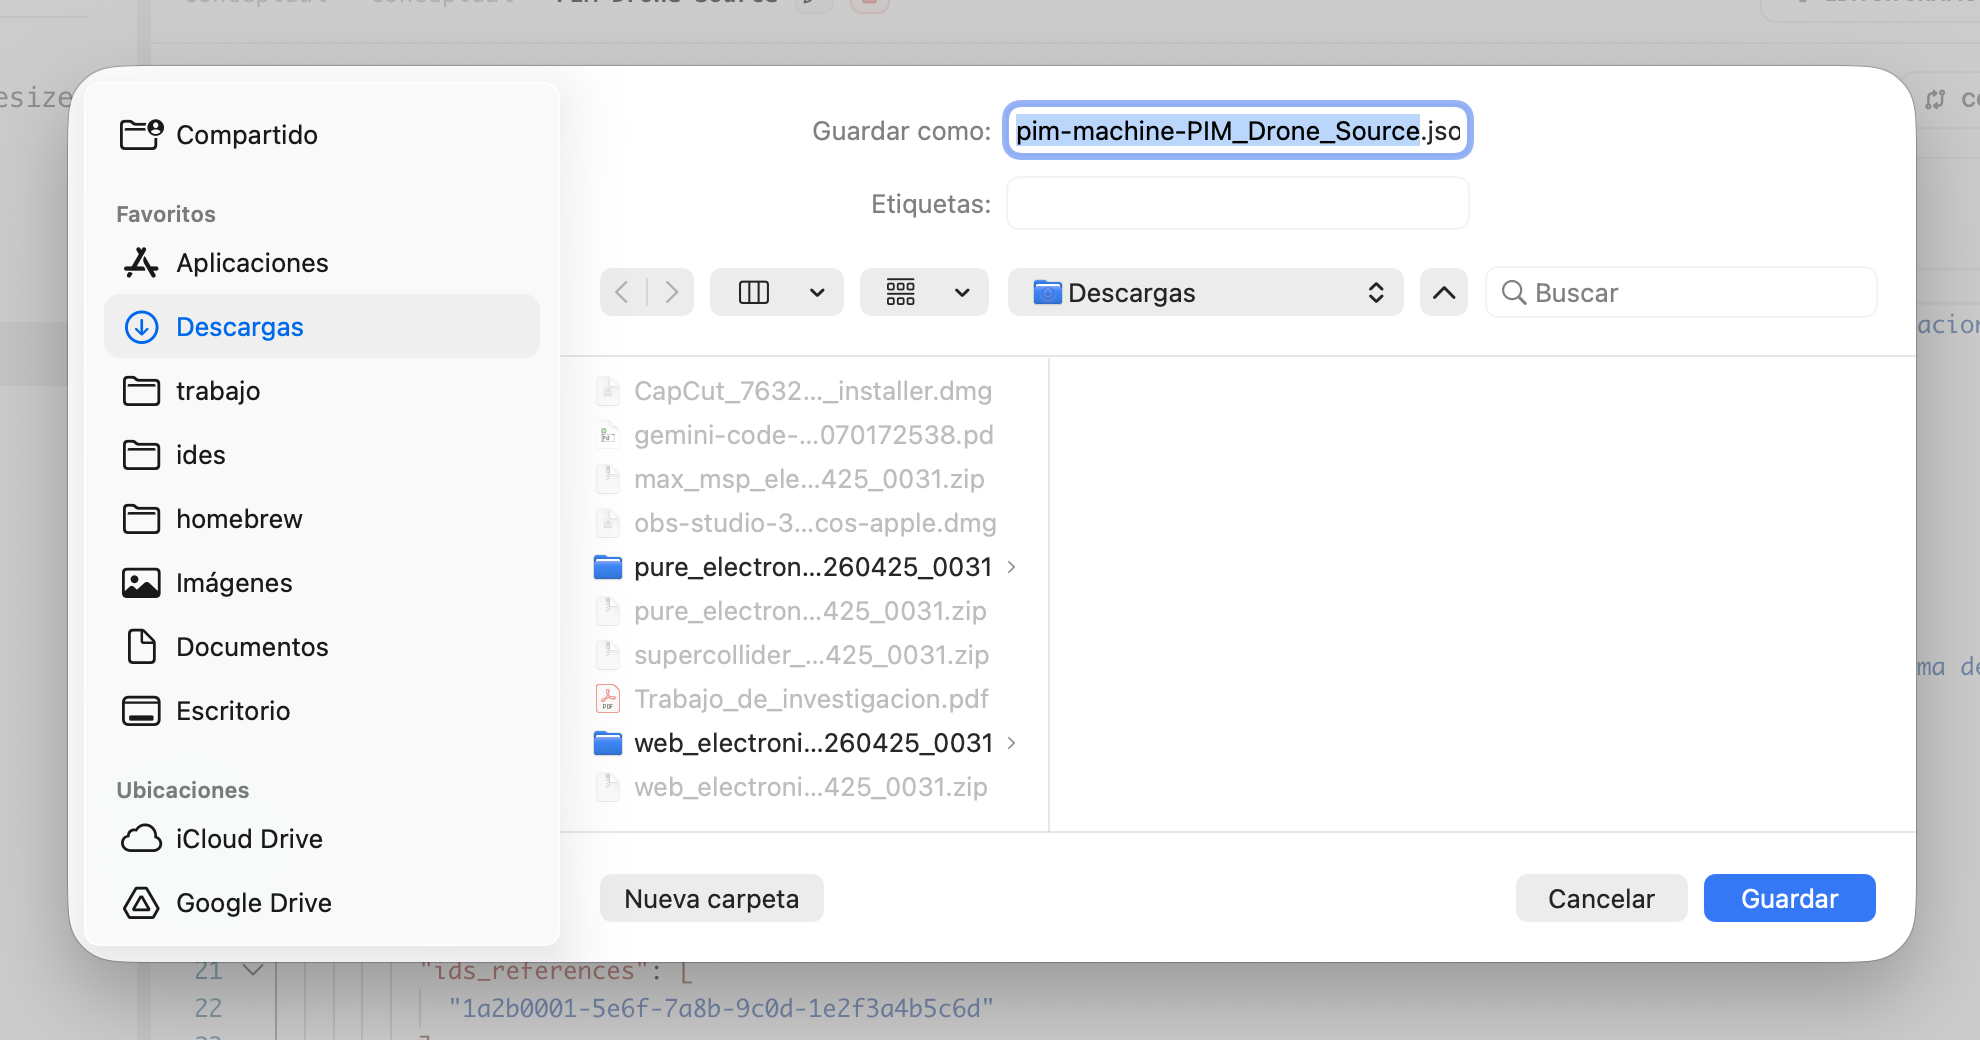
\includegraphics[width=0.6\textwidth]{imagenes/06_diseno/20_exportarJsonMaquinaPim.png}
    \caption{Exportación individual del código fuente de la máquina PIM.}
\end{figure}

Las herramientas de auditoría visual (\textit{diff}) y las capacidades de exportación se aplican también a nivel de máquina, proveyendo al arquitecto de software un control absoluto sobre el ciclo de vida del diseño computacional de cada componente.
